\documentclass[svgnames,smaller,table]{beamer}
\usepackage{multirow}
\usepackage{tikz}
\usefonttheme[onlymath]{serif}

\usepackage{listings}
% Configura o listings
\lstset{
  %  basicstyle=\footnotesize,\small,...\tiny
  basicstyle=\ttfamily\scriptsize,
  commentstyle=\color{mygreen},
  numbers=left,
  stepnumber=1,
  showstringspaces=false,
  tabsize=2,
  breaklines=true,
  breakatwhitespace=false
 columns=fixed,
 fontadjust=true,
 basewidth=0.5em
}


\usetheme{lthn}
\setbeamercolor*{normal text}{fg=black}
% -----------------------------------------------------------------------------------------------------------------

\title[Slide]{AUNIRA 2019 e perspectivas para imageamento por nêutrons no CDTN}
\author{Vitor Vasconcelos A. Silva}
\date{\today}
\institute{%
  LTHN - Laboratório de Termo-hidráulica e Neutrônica
  \par
  Serviço de Tecnologia de Reatores - CDTN/CNEN}

\begin{document}

%-------------------------------------------------
\begin{frame}
\titlepage
\end{frame}

%-------------------------------------------------
\begin{frame}
  \frametitle{Summary}
  \tableofcontents%[pausesections]
\end{frame}


\section{AUNIRA 2019}
%-------------------------------------------------
\begin{frame}
  \frametitle{AUNIRA 2019 - Daejeon, República da Coréia}
  \framesubtitle{Advanced Use of Neutron Imaging for Research and Applications}
  \begin{center}
    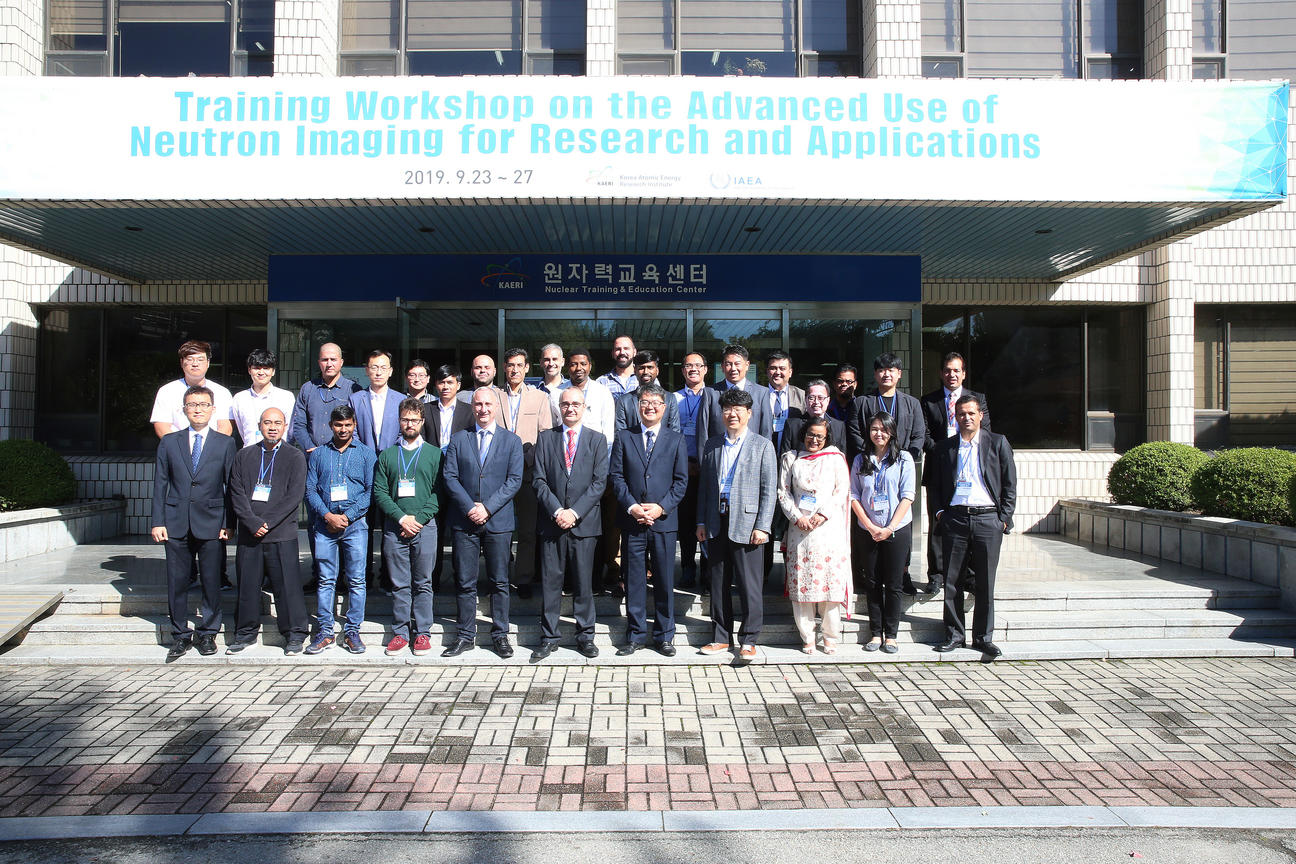
\includegraphics[scale=0.25]{figures/grupo.jpg}
    \end{center}
\end{frame}

%-------------------------------------------------
\begin{frame}
  \frametitle{AUNIRA 2019 - Daejeon, República da Coréia}
  \framesubtitle{Advanced Use of Neutron Imaging for Research and Applications}
  \begin{itemize}
  \item 2019: foco em aplicações de  Herança Cultural
  \item Anfitriões: KAERI (Korea Atomic Energy Research Institute)
  \item 21 participantes de 18 países
  \item Duração de uma semana (segunda até meio-dia de sexta-feira)
  \end{itemize}
  Formato:
  \begin{enumerate}
  \item Apresentações
  \item Visita técnica às instalações do reator HANARO
  \item Uma seção prática: uso do software \textit{VG Studio}\textcopyright
  \item Seção de posters
  \end{enumerate}

\end{frame}

%-------------------------------------------------
\begin{frame}
  \frametitle{AUNIRA 2019 - Daejeon, República da Coréia}
  \framesubtitle{Advanced Use of Neutron Imaging for Research and Applications}
  \begin{center}
    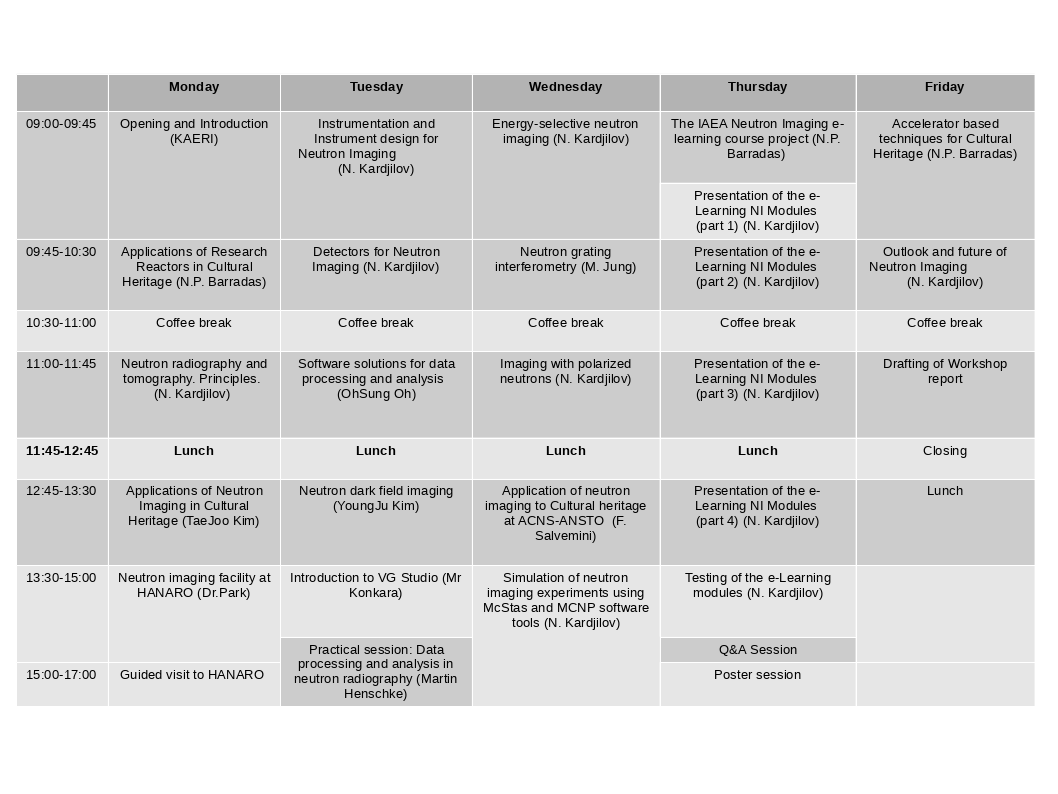
\includegraphics[scale=2.0]{figures/agenda.png}
    \end{center}
\end{frame}

%-------------------------------------------------
\begin{frame}
  \frametitle{AUNIRA 2019 - Daejeon, República da Coréia}
  \framesubtitle{Advanced Use of Neutron Imaging for Research and Applications}
  \begin{center}
    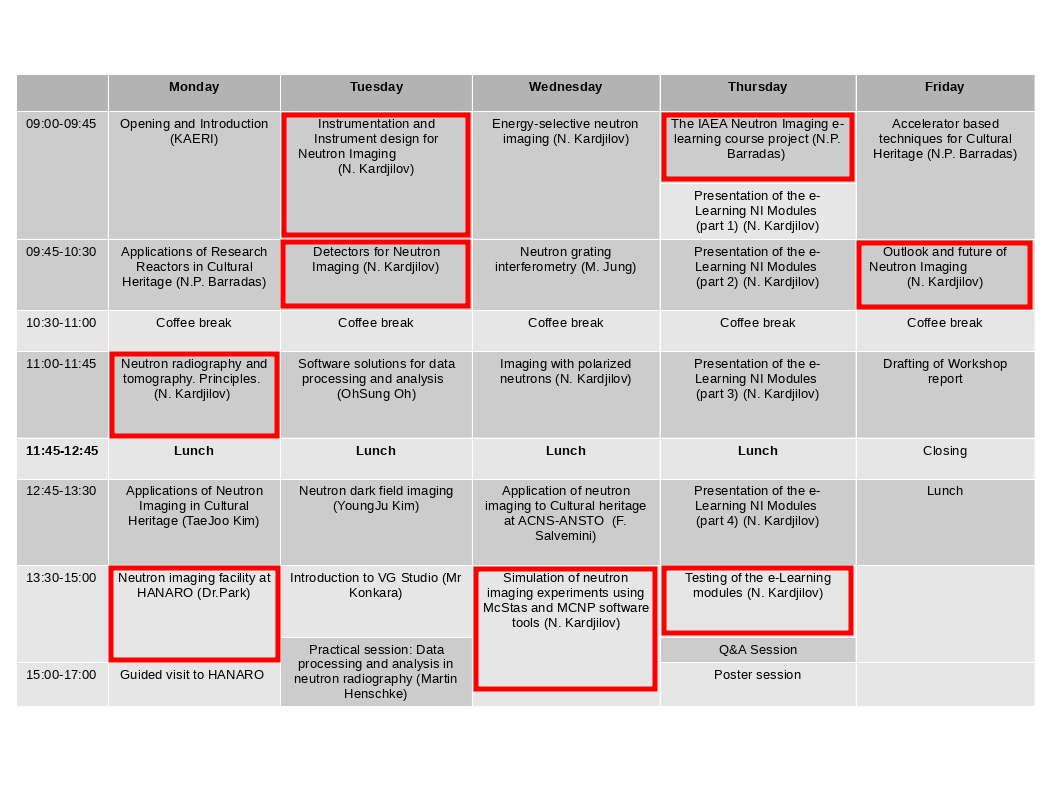
\includegraphics[scale=2.0]{figures/agenda-marked.png}
    \end{center}
\end{frame}

%-------------------------------------------------


\section{Apresentações escolhidas}
%-------------------------------------------------
\subsection{Neutron Radiography and Tomography: Principles}
%-------------------------------------------------
\begin{frame}
  \frametitle{Apresentações escolhidas}
  \framesubtitle{(1)}
  \begin{center}
    Neutron Radiography and Tomography: Principles\\
    \vspace{2.0cm}
    N. Kardjilov
  \end{center}
\end{frame}

\begin{frame}
  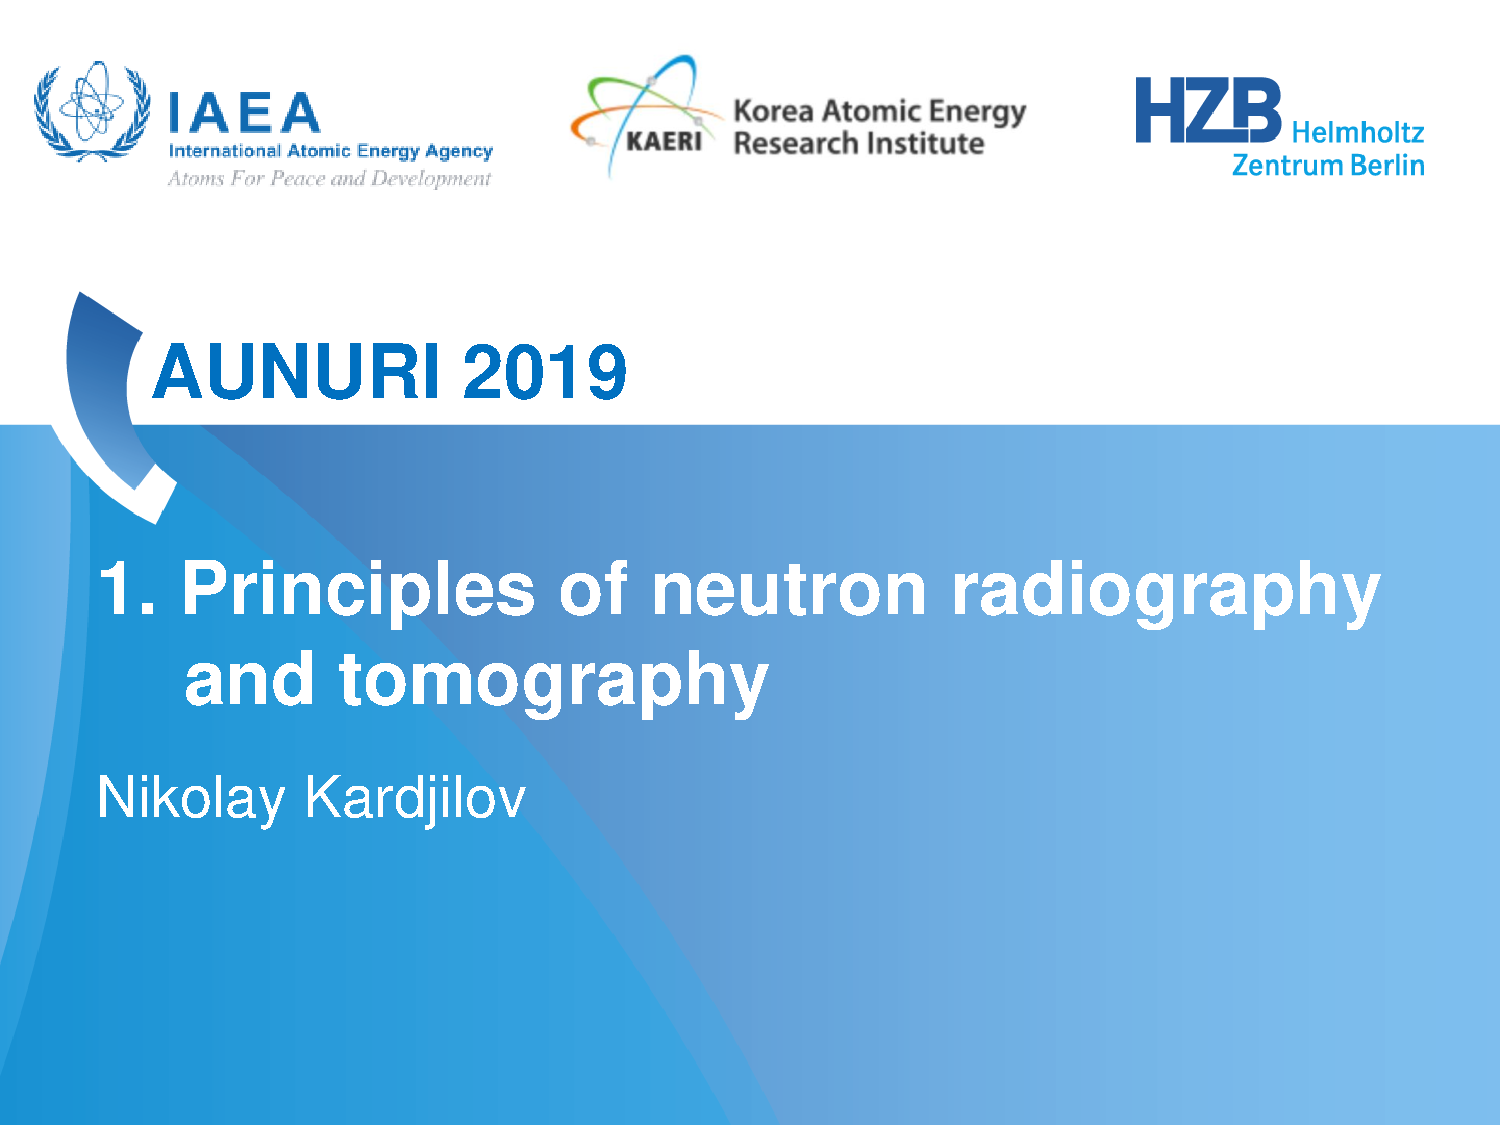
\includepdf{figures/pres1/sl1.pdf}
\end{frame}

\begin{frame}
  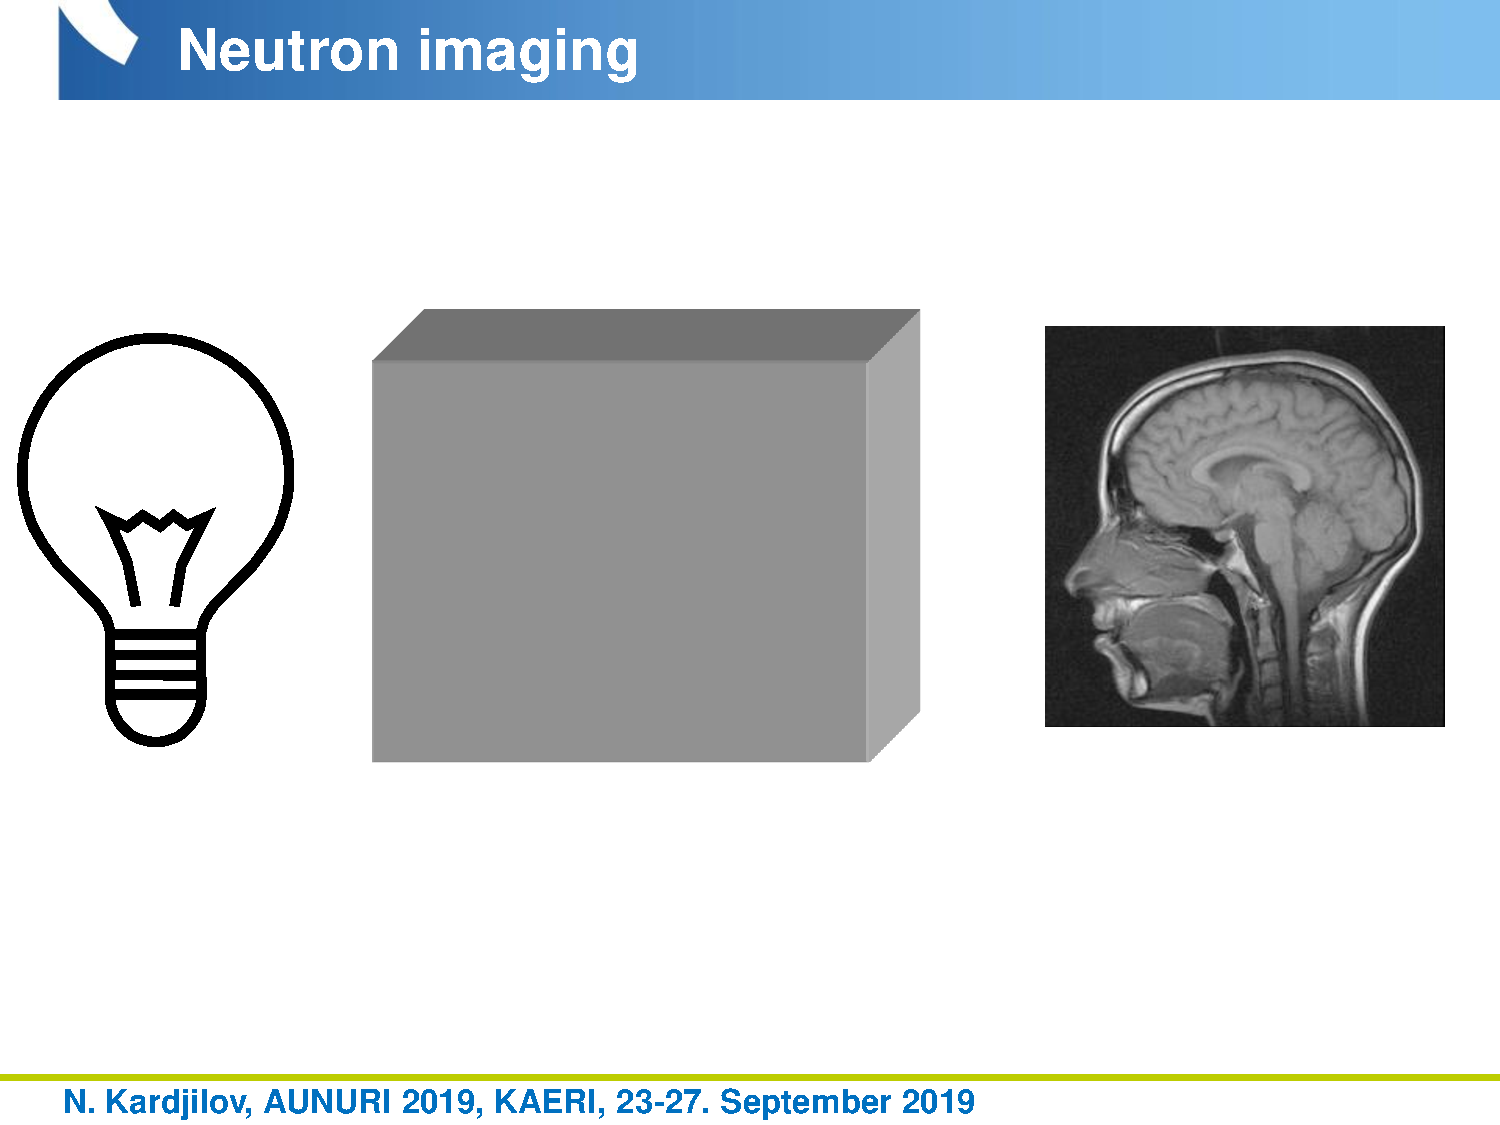
\includepdf{figures/pres1/sl5.pdf}
\end{frame}

\begin{frame}
    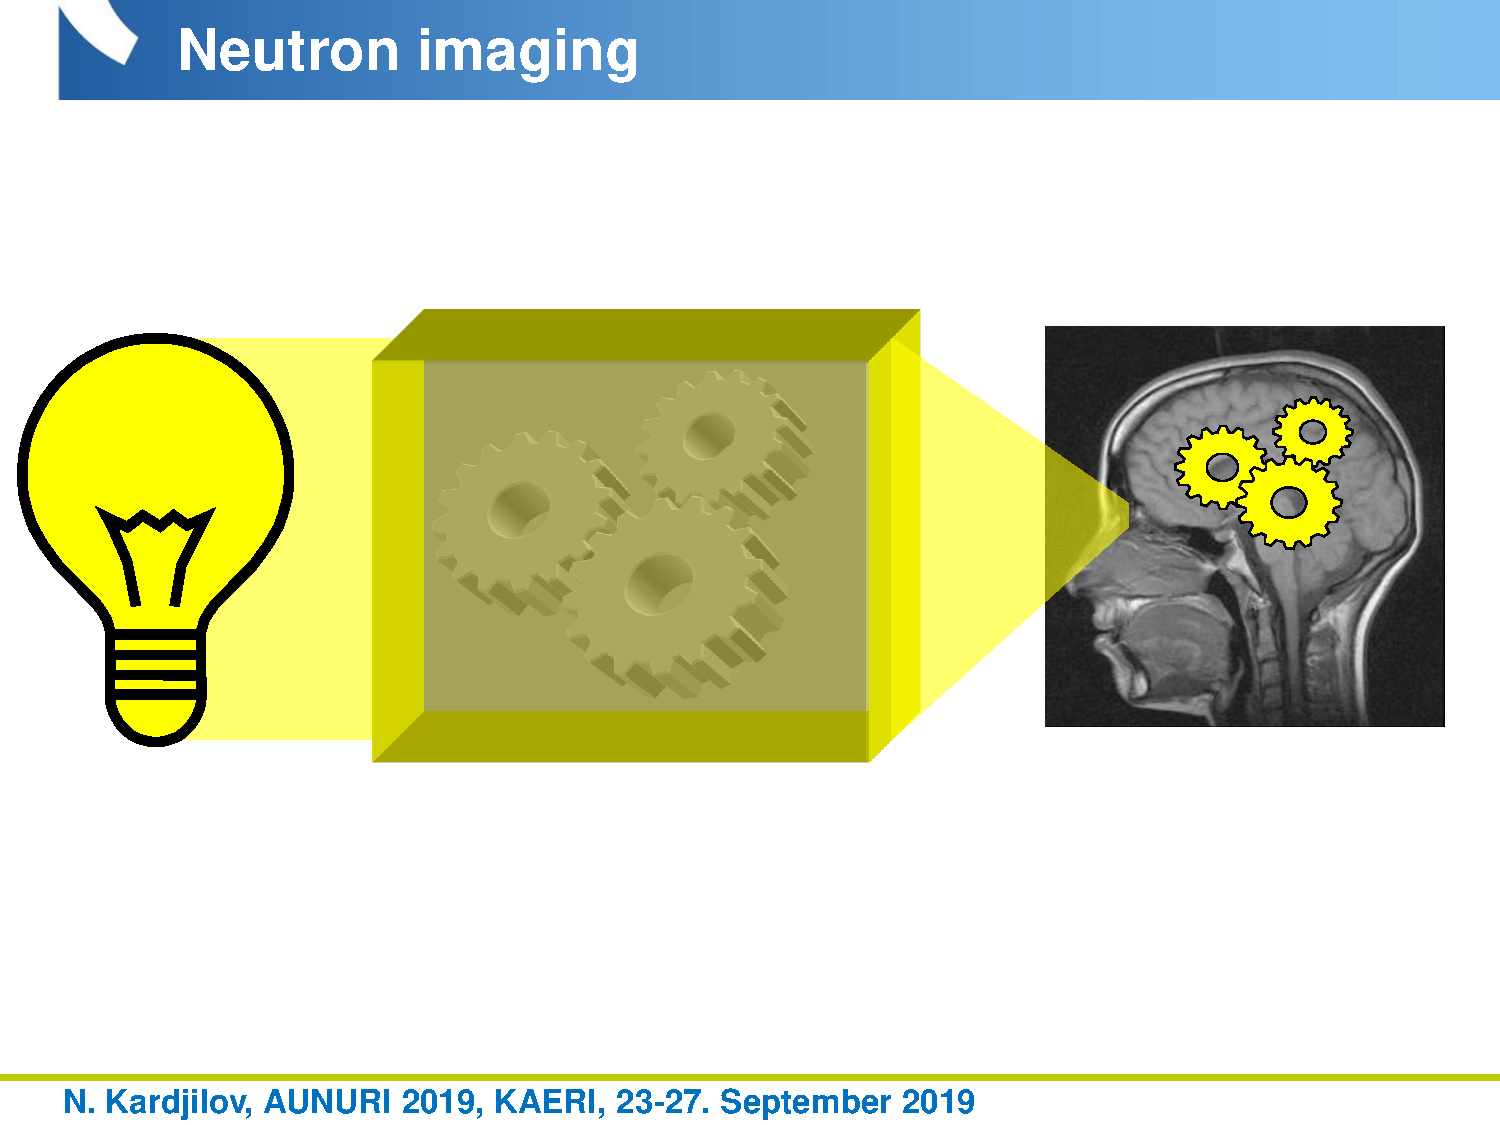
\includepdf{figures/pres1/sl6.pdf}
\end{frame}

\begin{frame}
  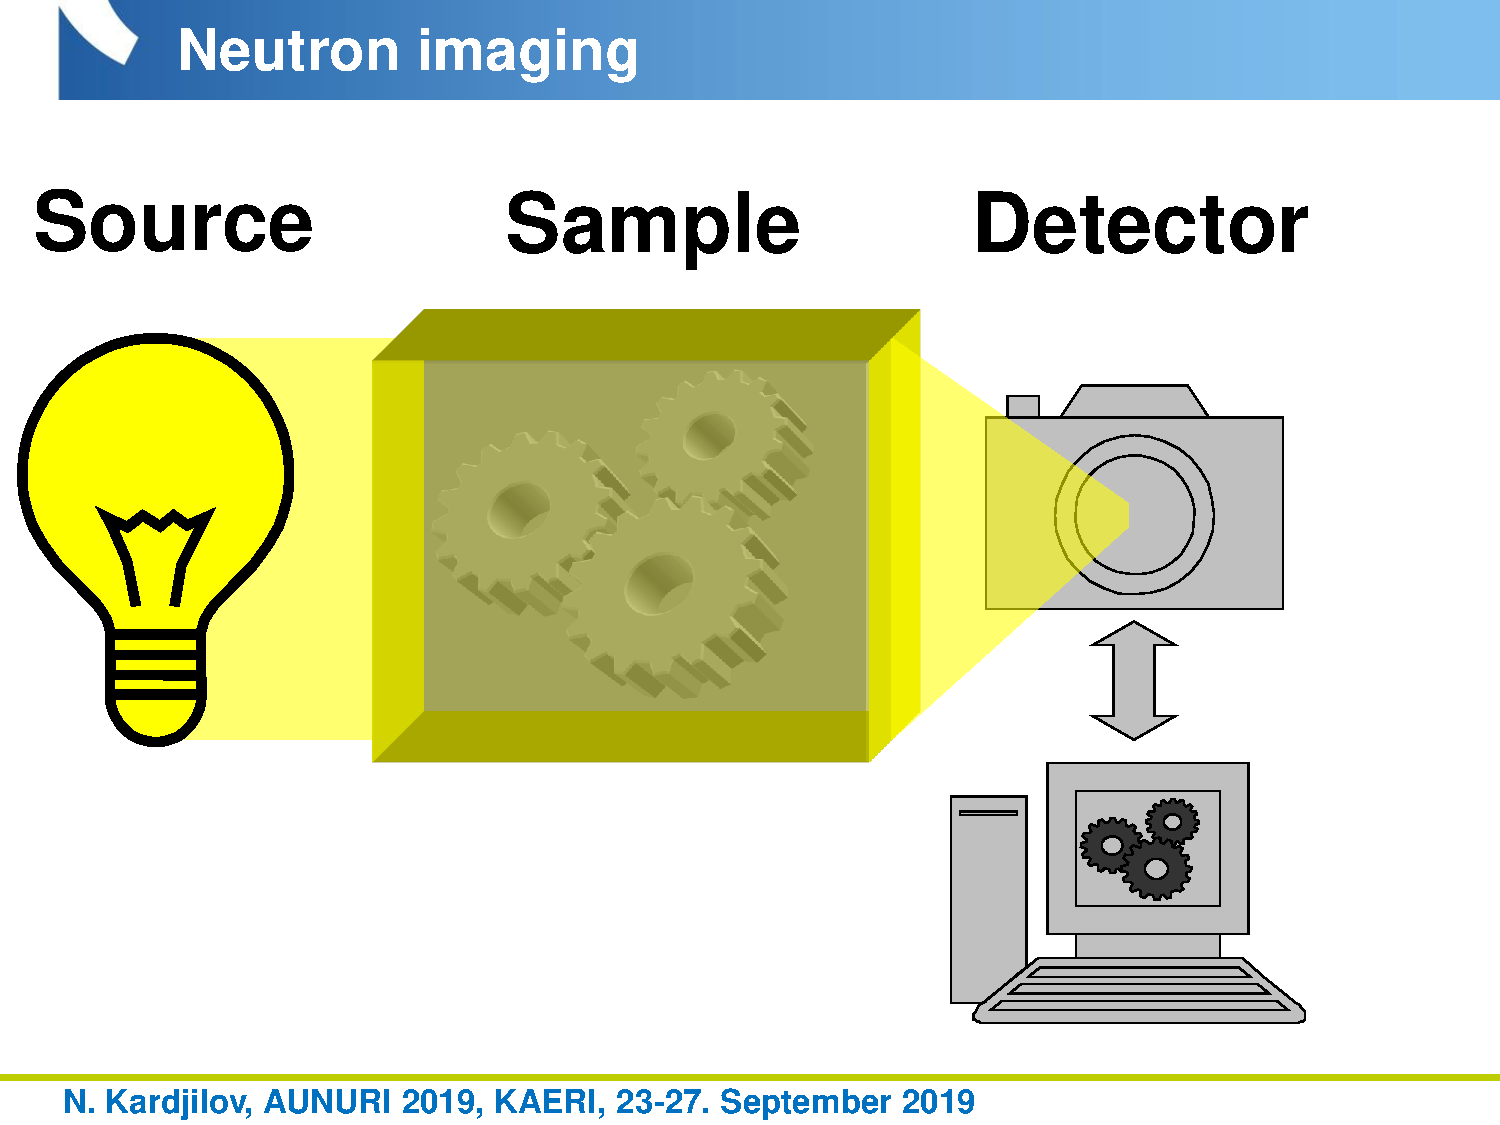
\includepdf{figures/pres1/sl7.pdf}
\end{frame}

\begin{frame}
  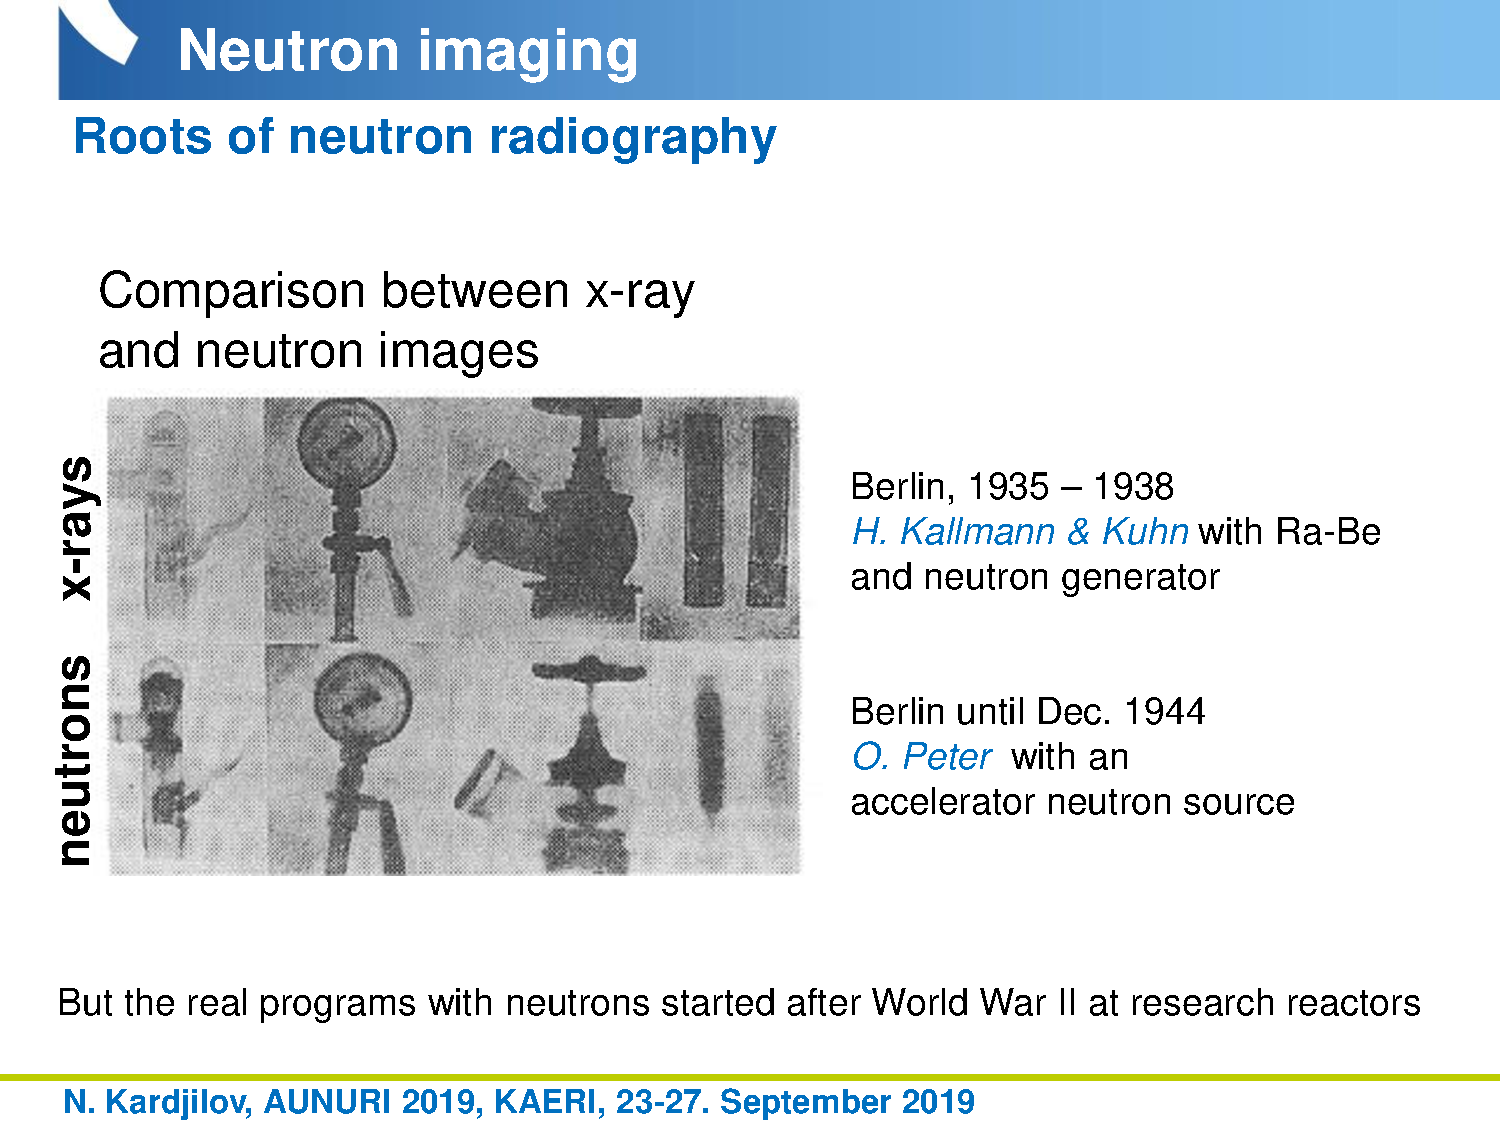
\includepdf{figures/pres1/sl10.pdf}
\end{frame}

\begin{frame}
  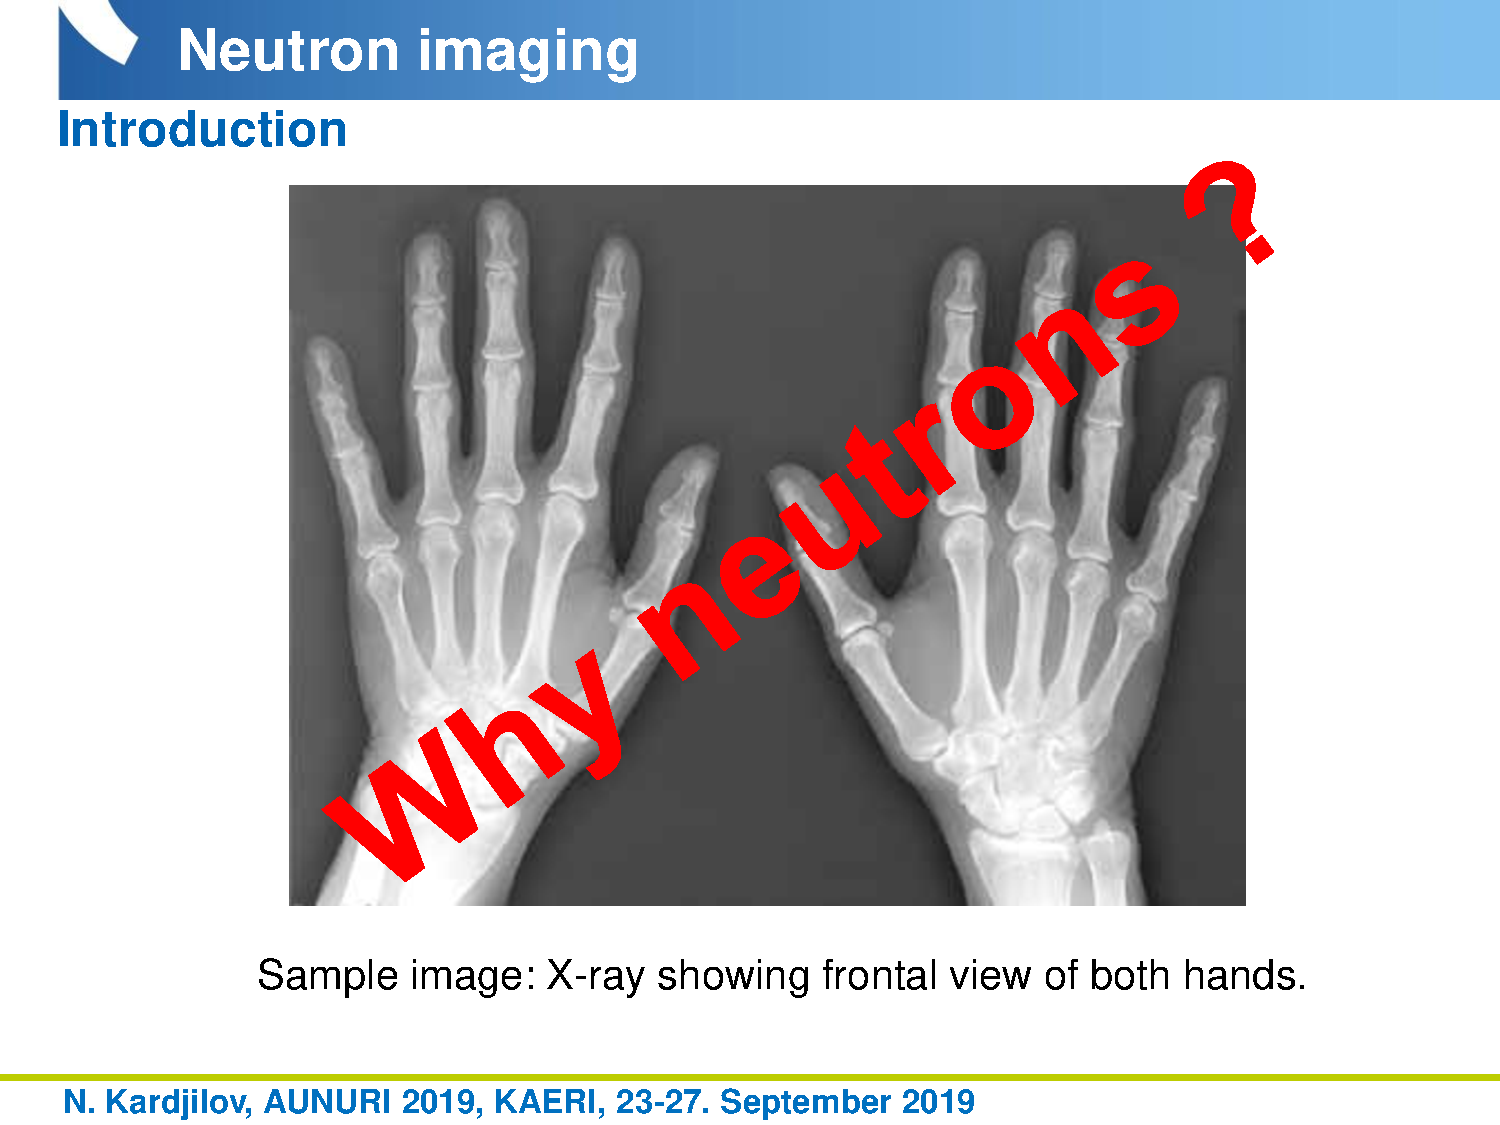
\includepdf{figures/pres1/sl11.pdf}
\end{frame}

\begin{frame}
  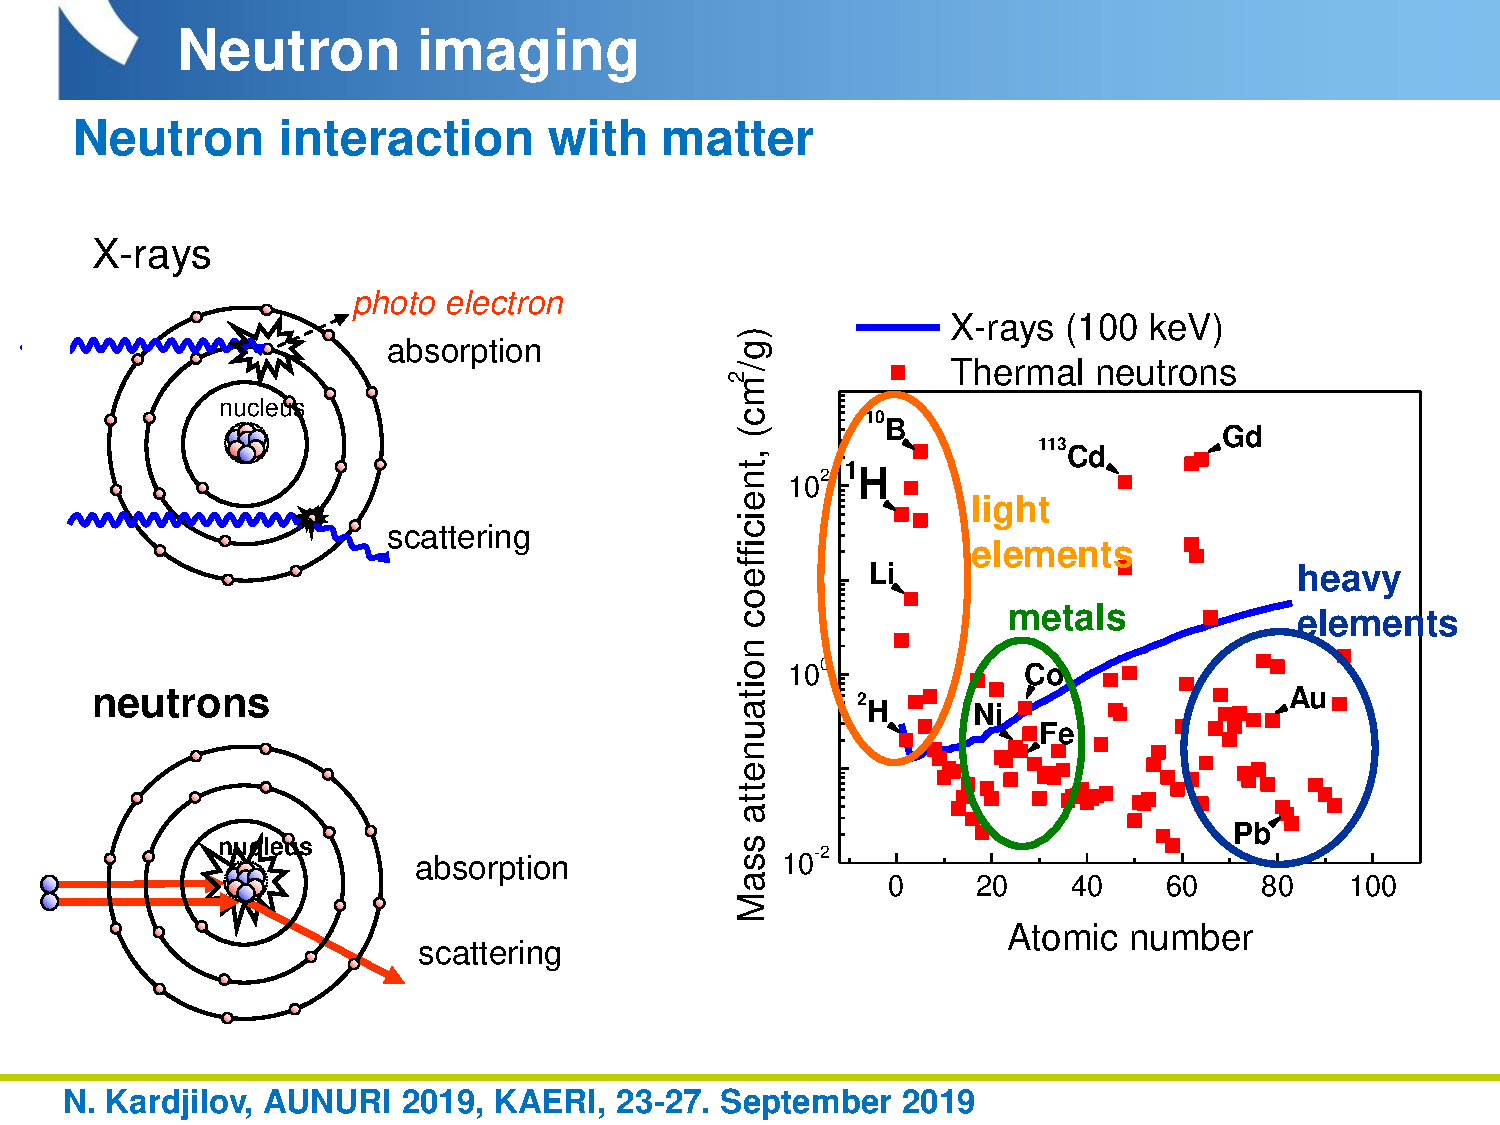
\includepdf{figures/pres1/sl12.pdf}
\end{frame}

\begin{frame}
  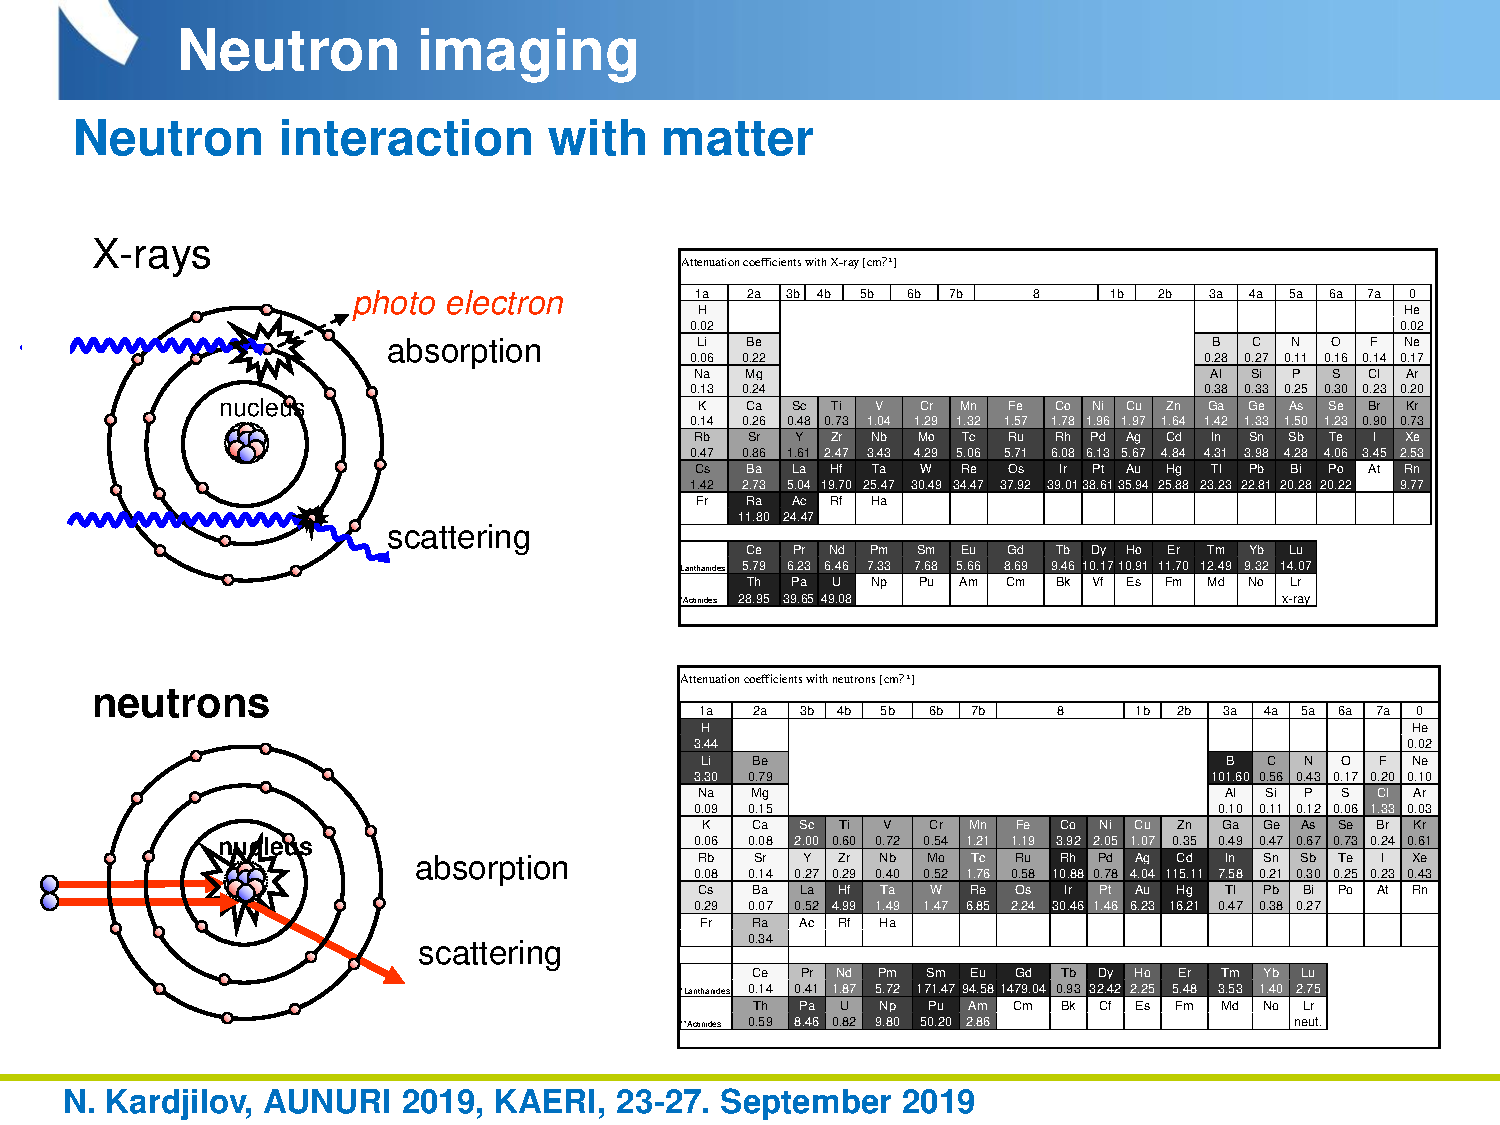
\includepdf{figures/pres1/sl13.pdf}
\end{frame}

\begin{frame}
  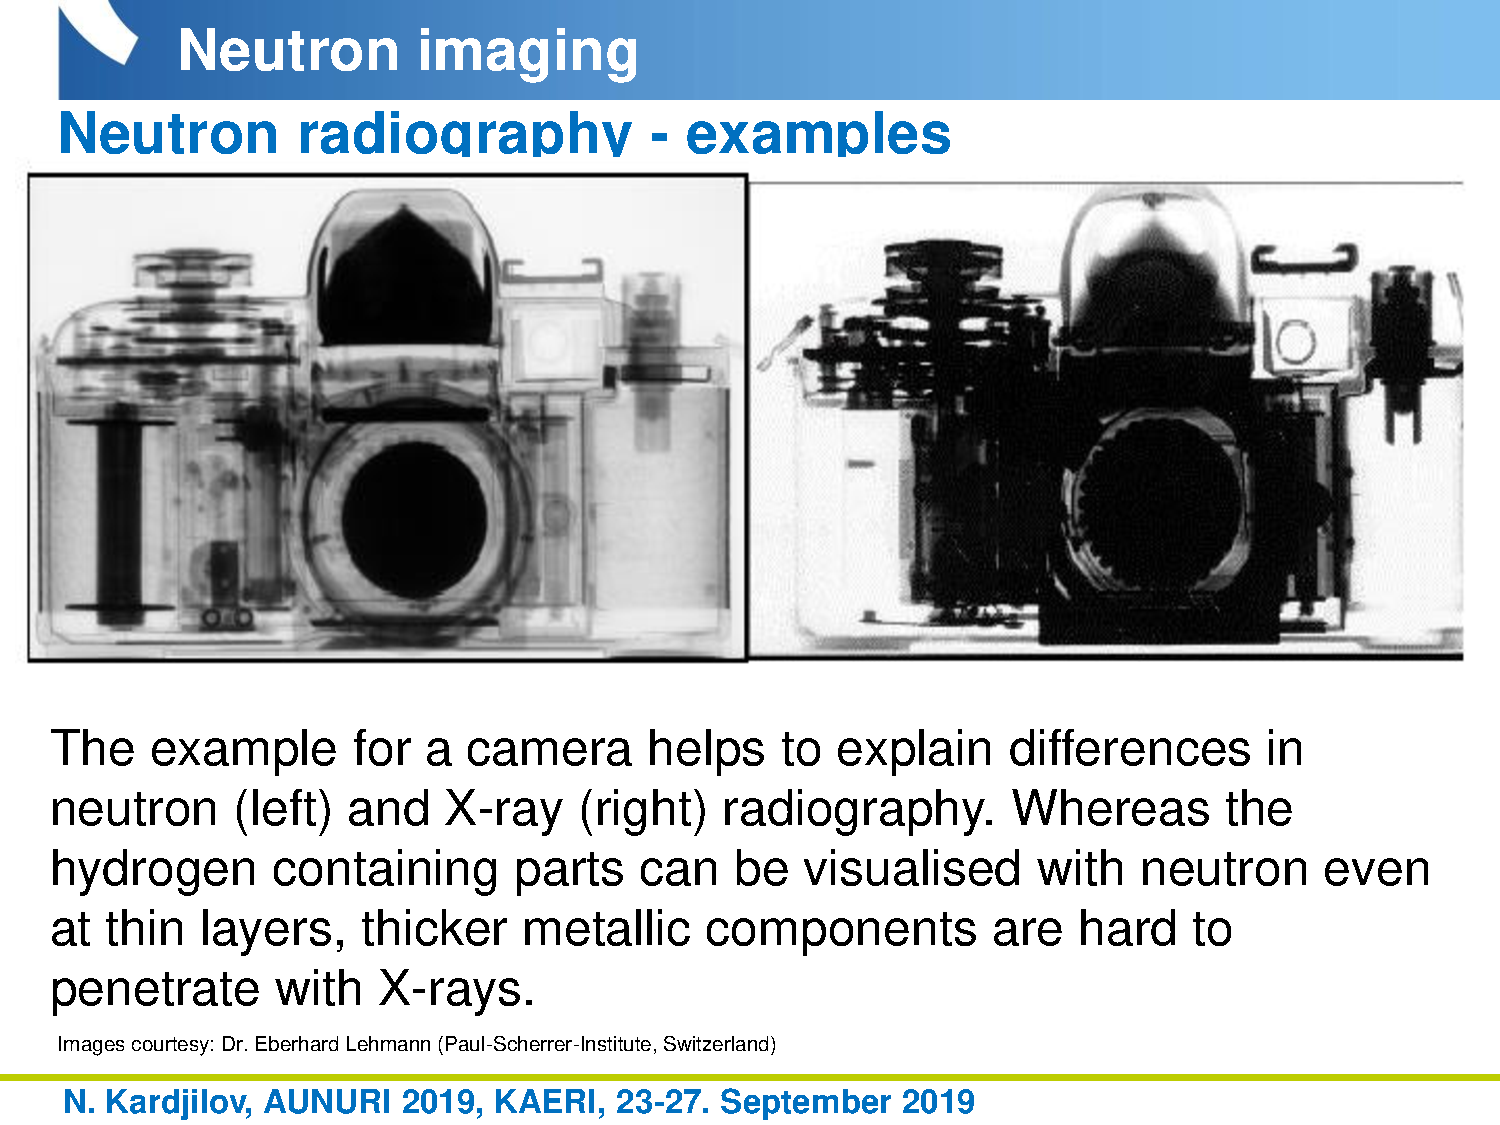
\includepdf{figures/pres1/sl14.pdf}
\end{frame}

%-------------------------------------------------
\subsection{Neutron Imaging Facility at HANARO}
%-------------------------------------------------
\begin{frame}
  \frametitle{Apresentações escolhidas}
  \framesubtitle{(2)}
  \begin{center}
    Neutron Imaging Facility at HANARO\\
    \vspace{2.0cm}
    Dr. Park
  \end{center}
\end{frame}


\begin{frame}
  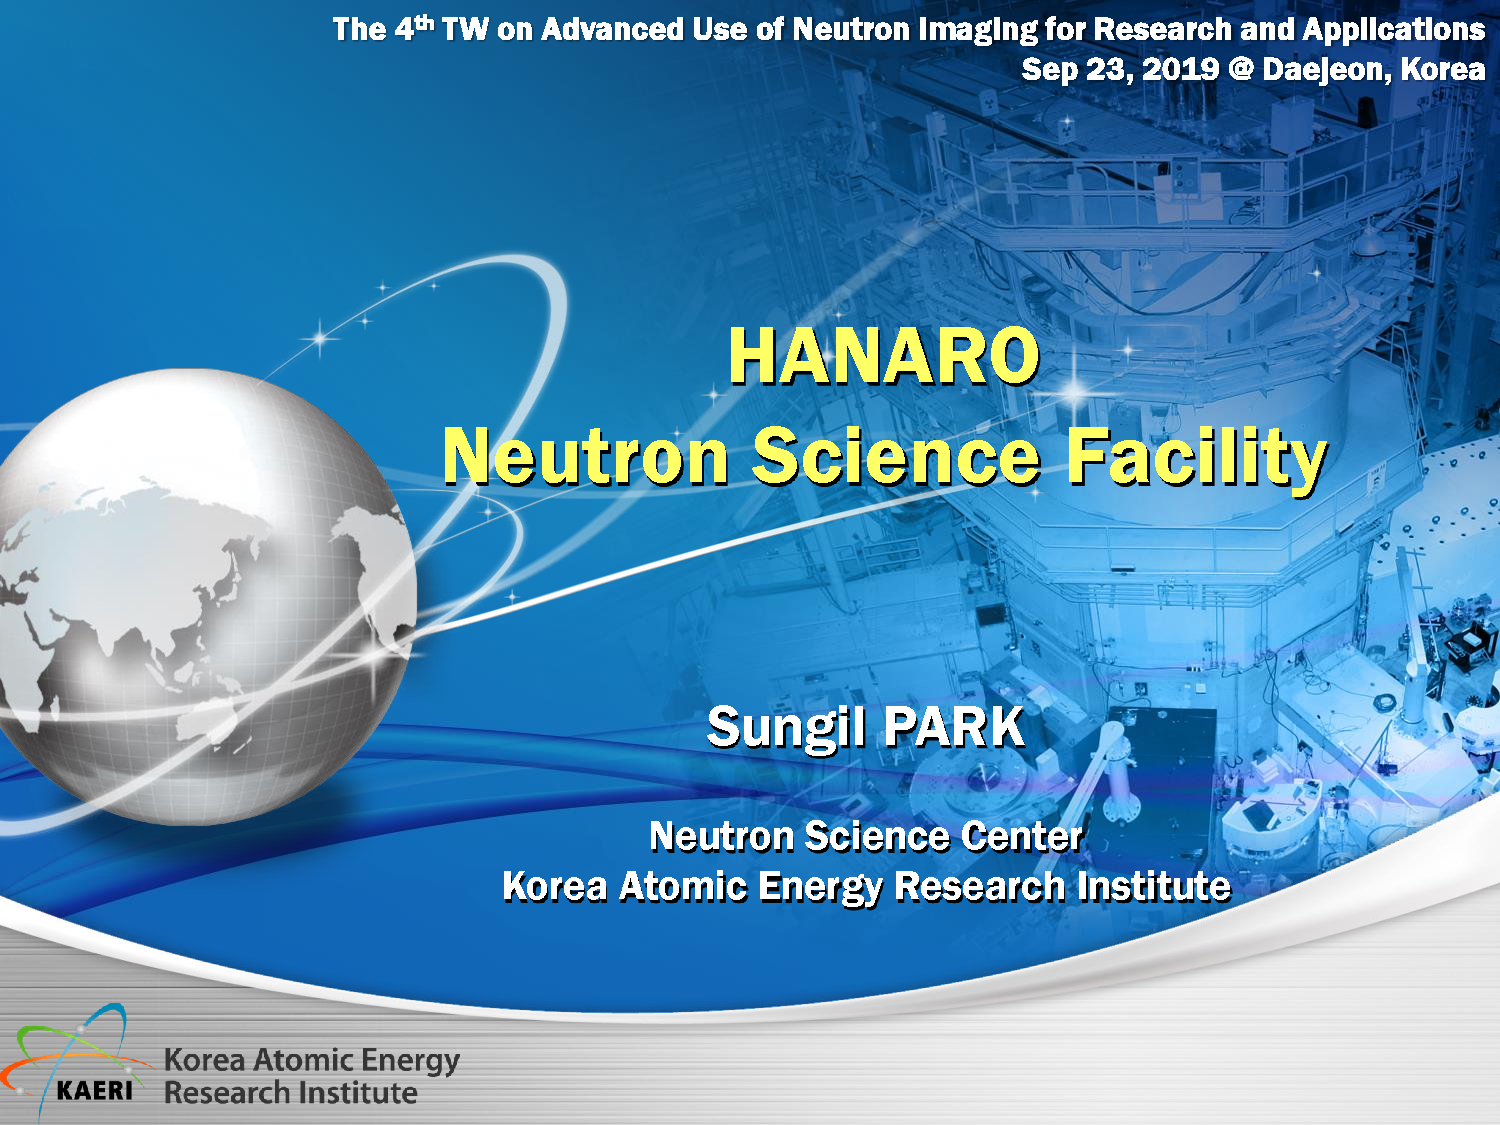
\includepdf{figures/pres2/sl-1.pdf}
\end{frame}

\begin{frame}
  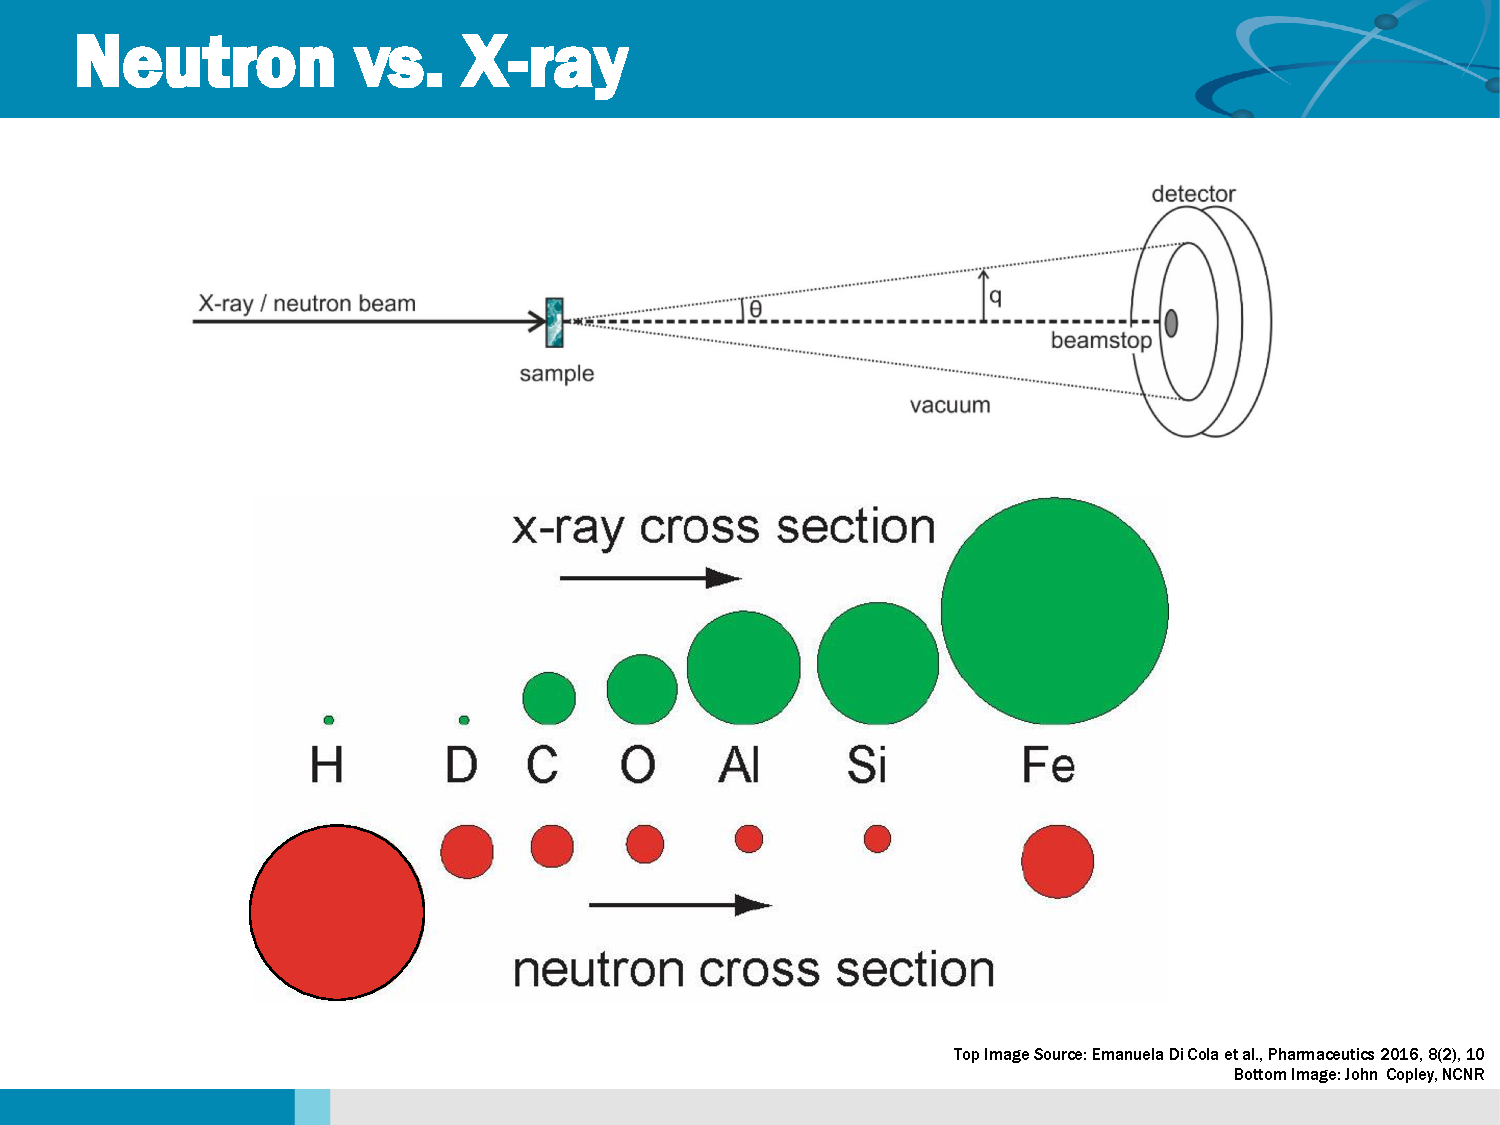
\includepdf{figures/pres2/sl-3.pdf}
\end{frame}

\begin{frame}
    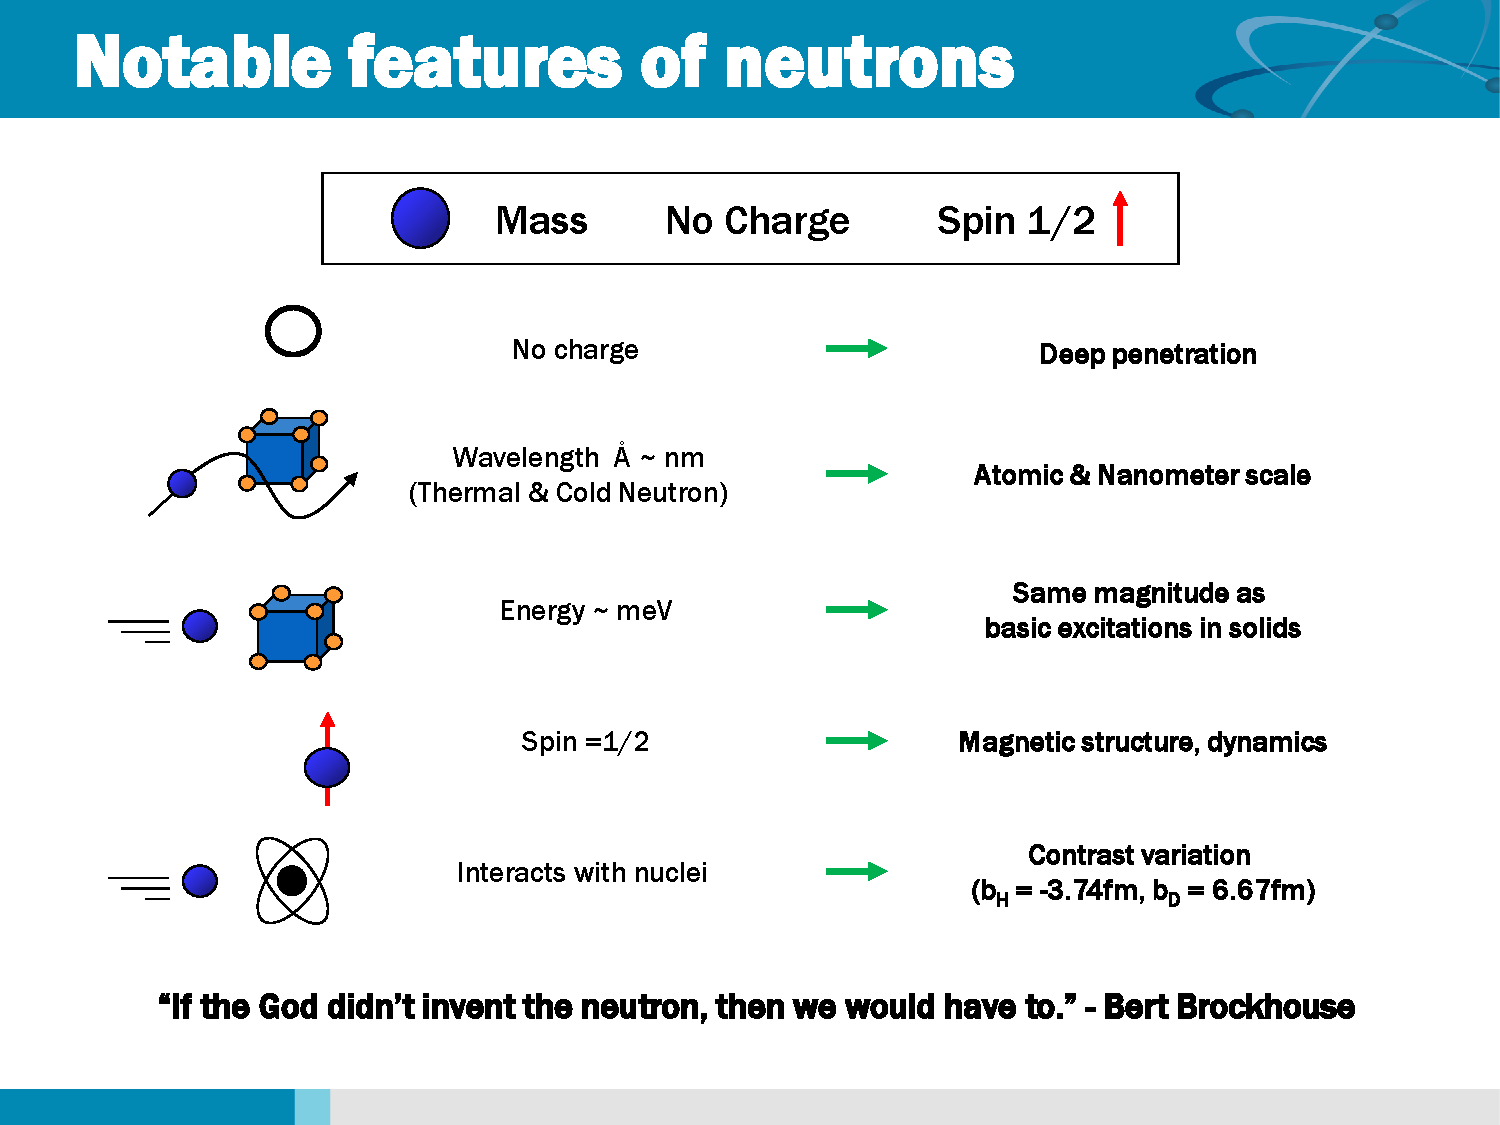
\includepdf{figures/pres2/sl-4.pdf}
\end{frame}

\begin{frame}
  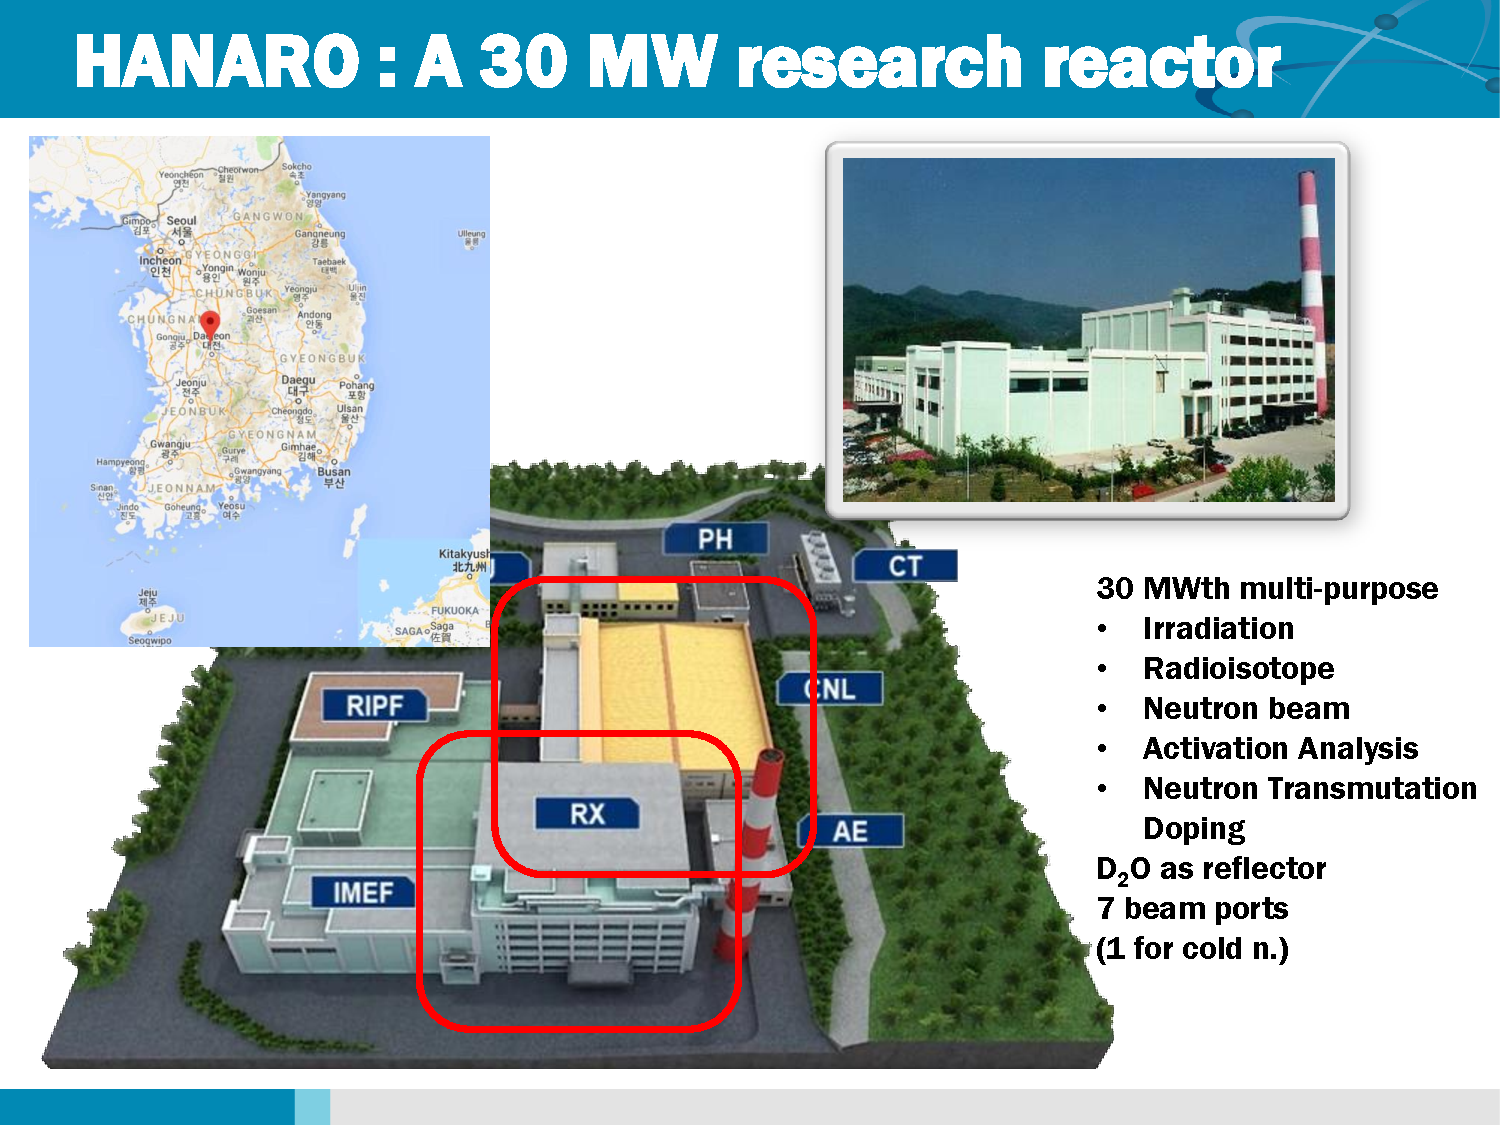
\includepdf{figures/pres2/sl-10.pdf}
\end{frame}

\begin{frame}
  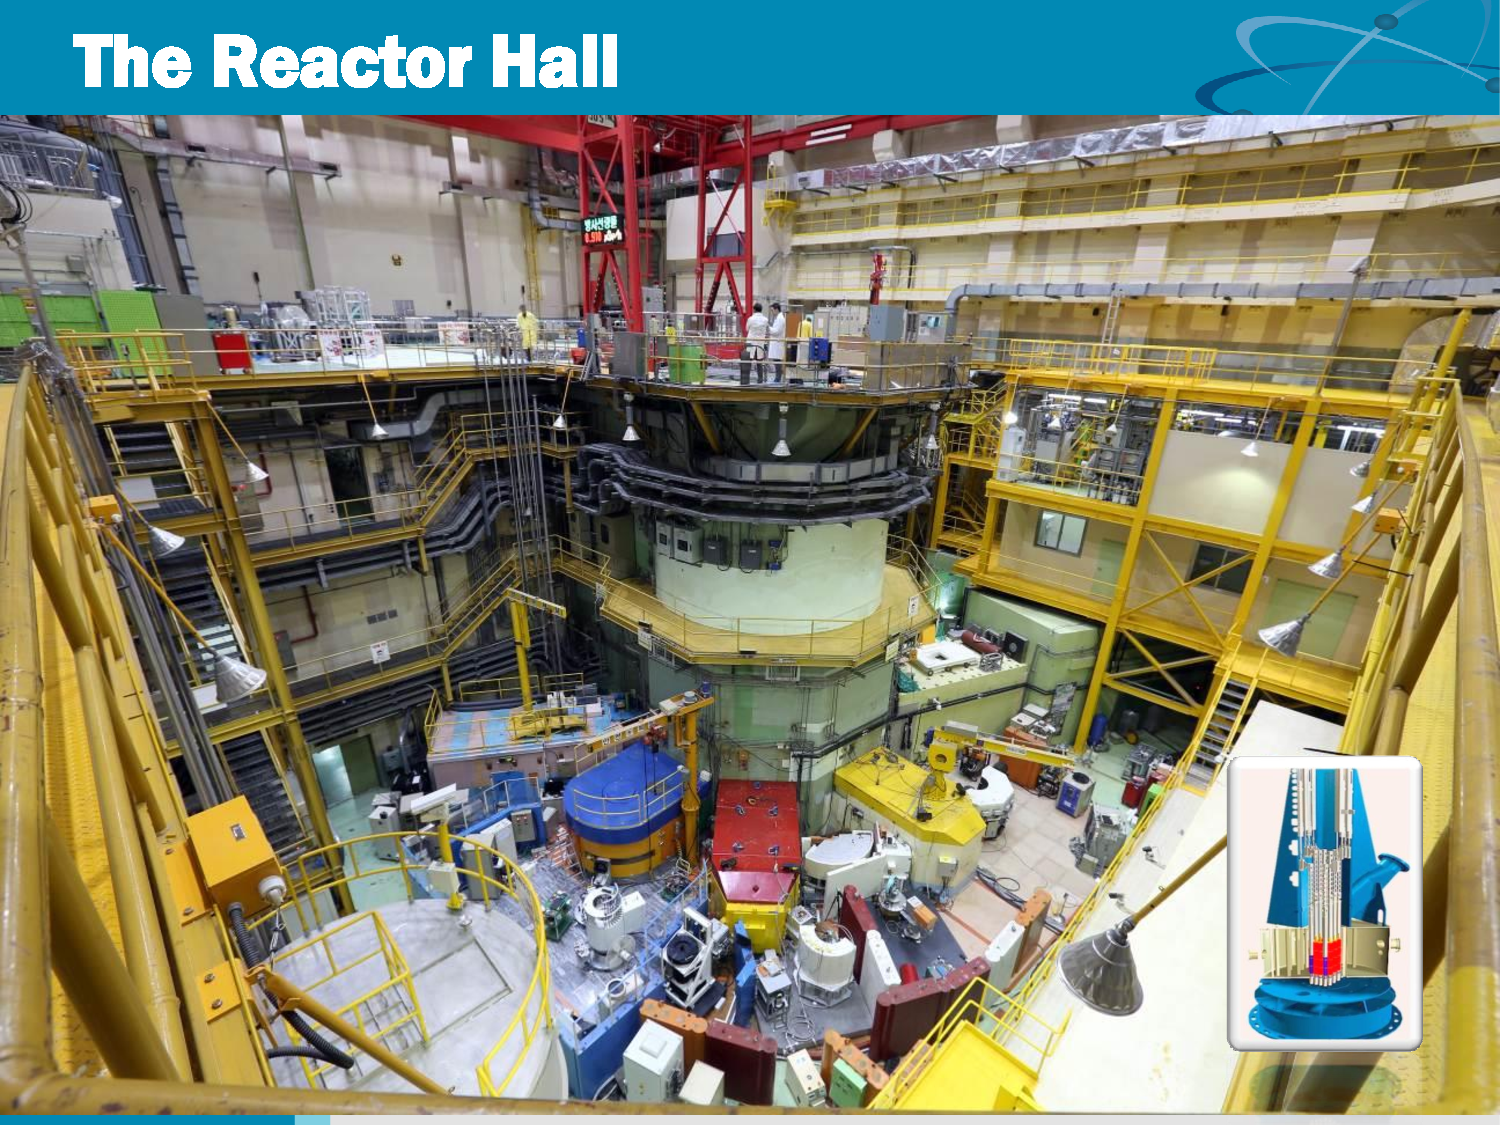
\includepdf{figures/pres2/sl-11.pdf}
\end{frame}

\begin{frame}
  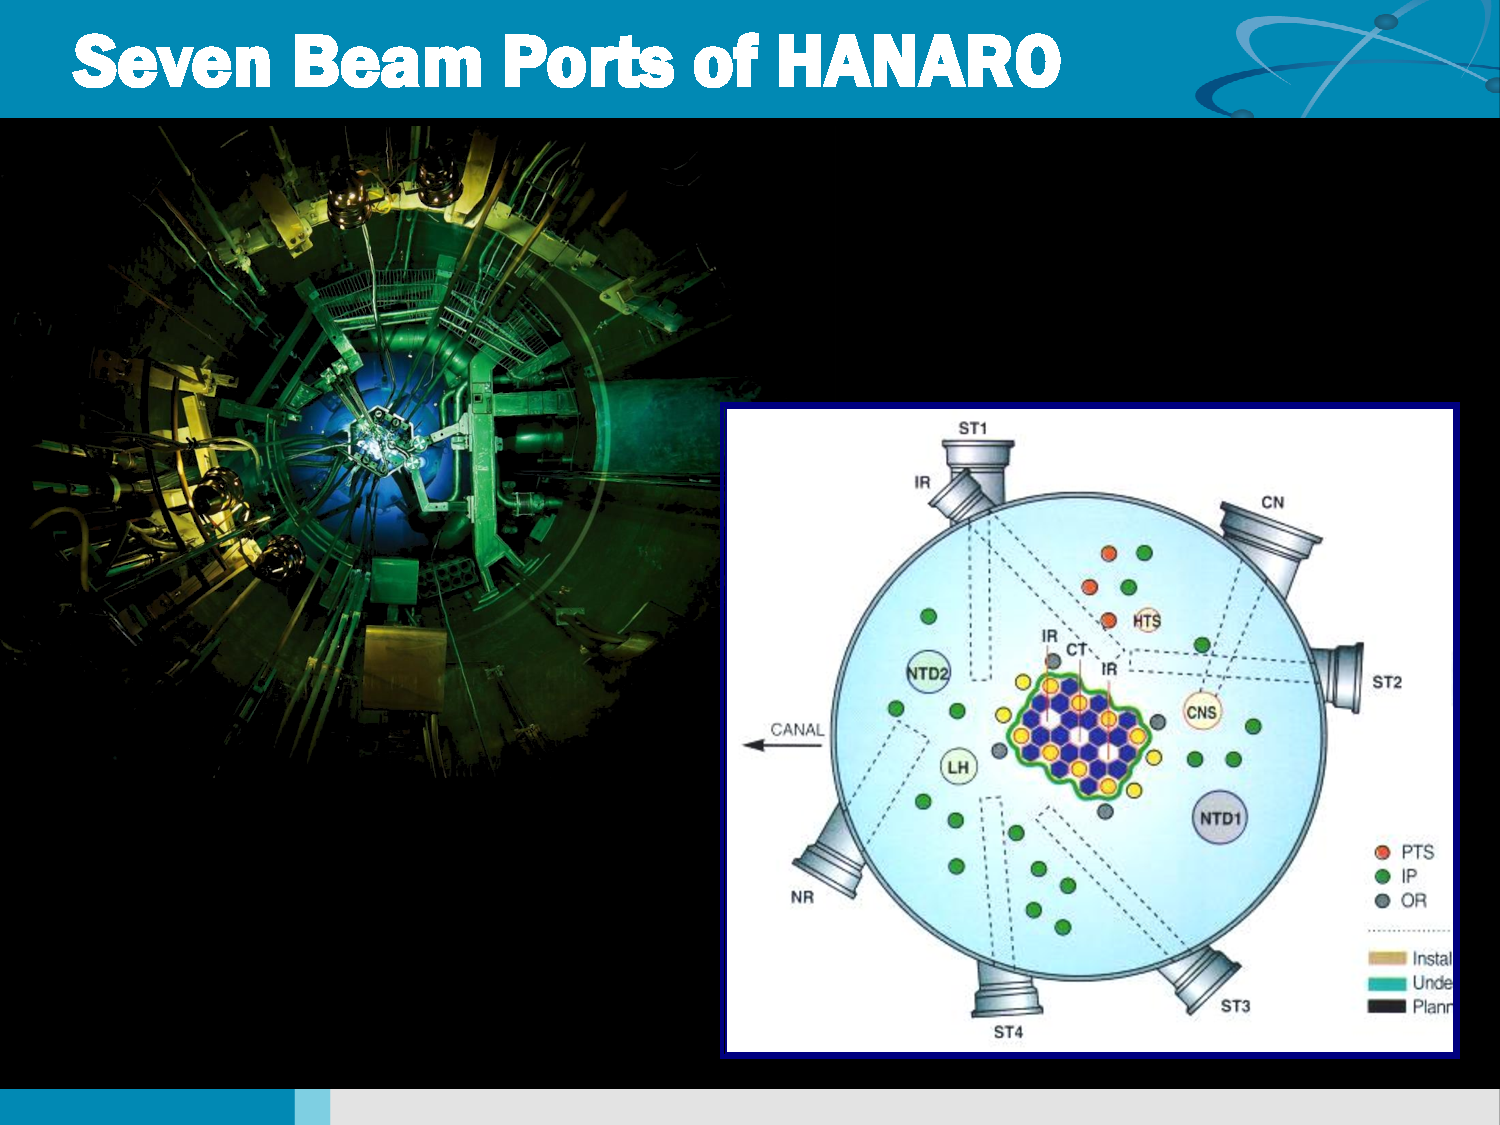
\includepdf{figures/pres2/sl-12.pdf}
\end{frame}

\begin{frame}
  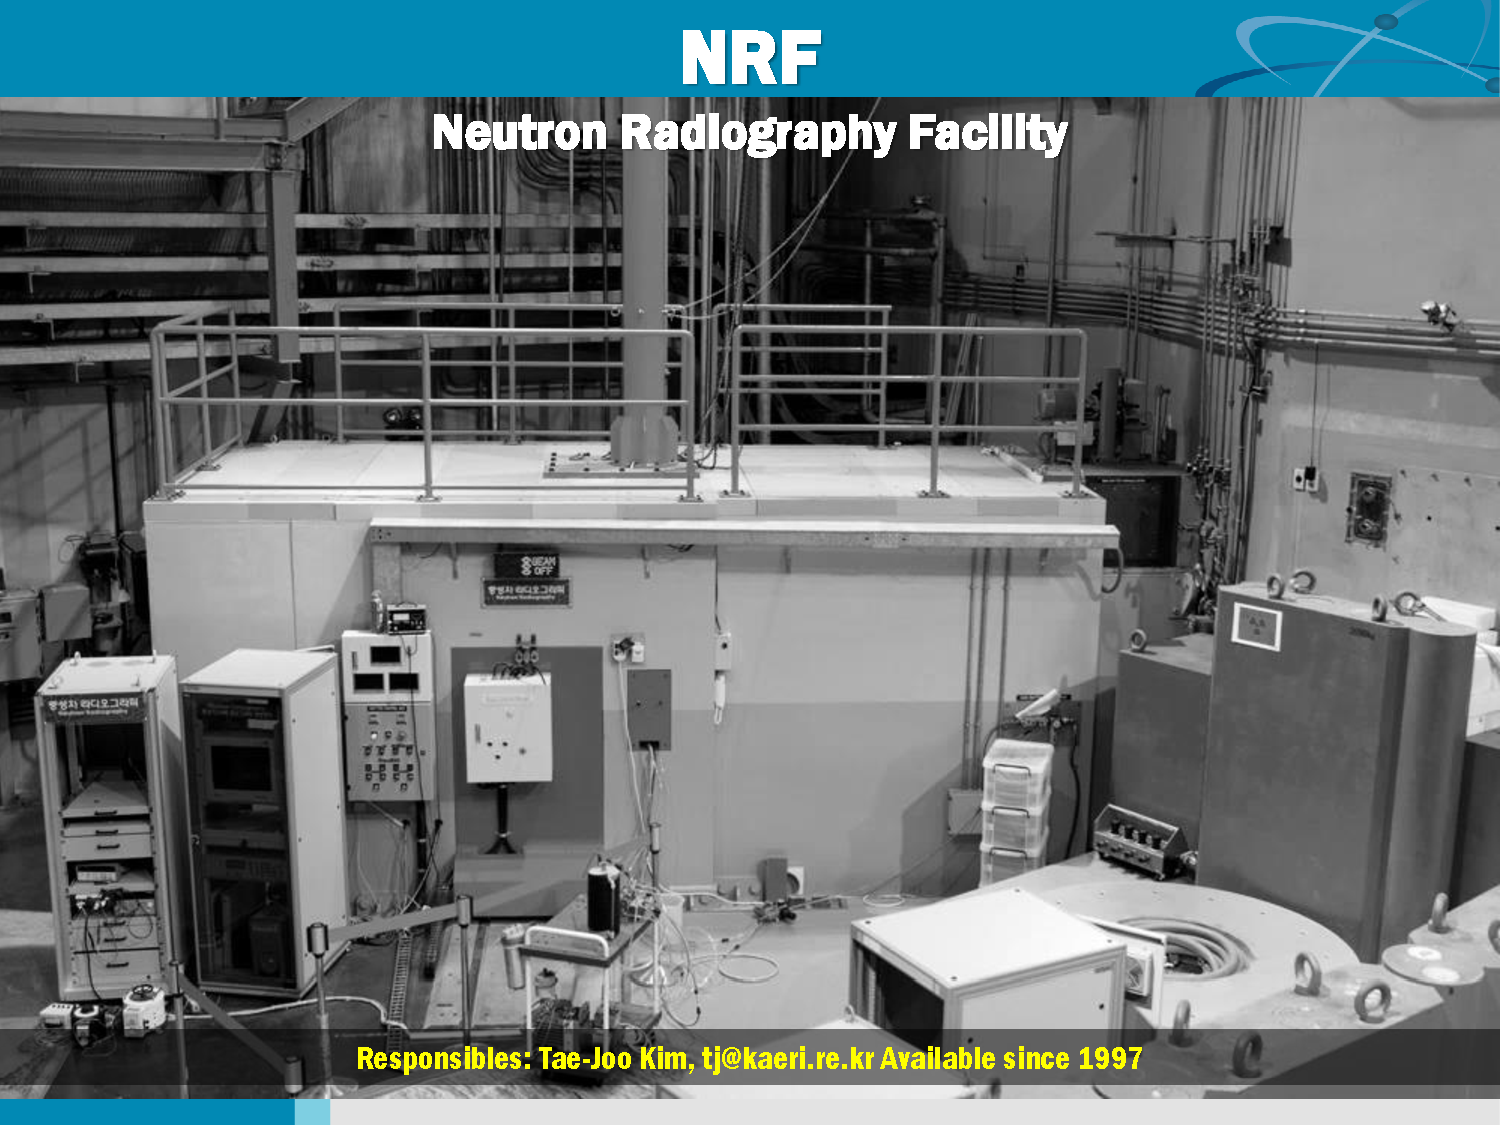
\includepdf{figures/pres2/sl-32.pdf}
\end{frame}

\begin{frame}
  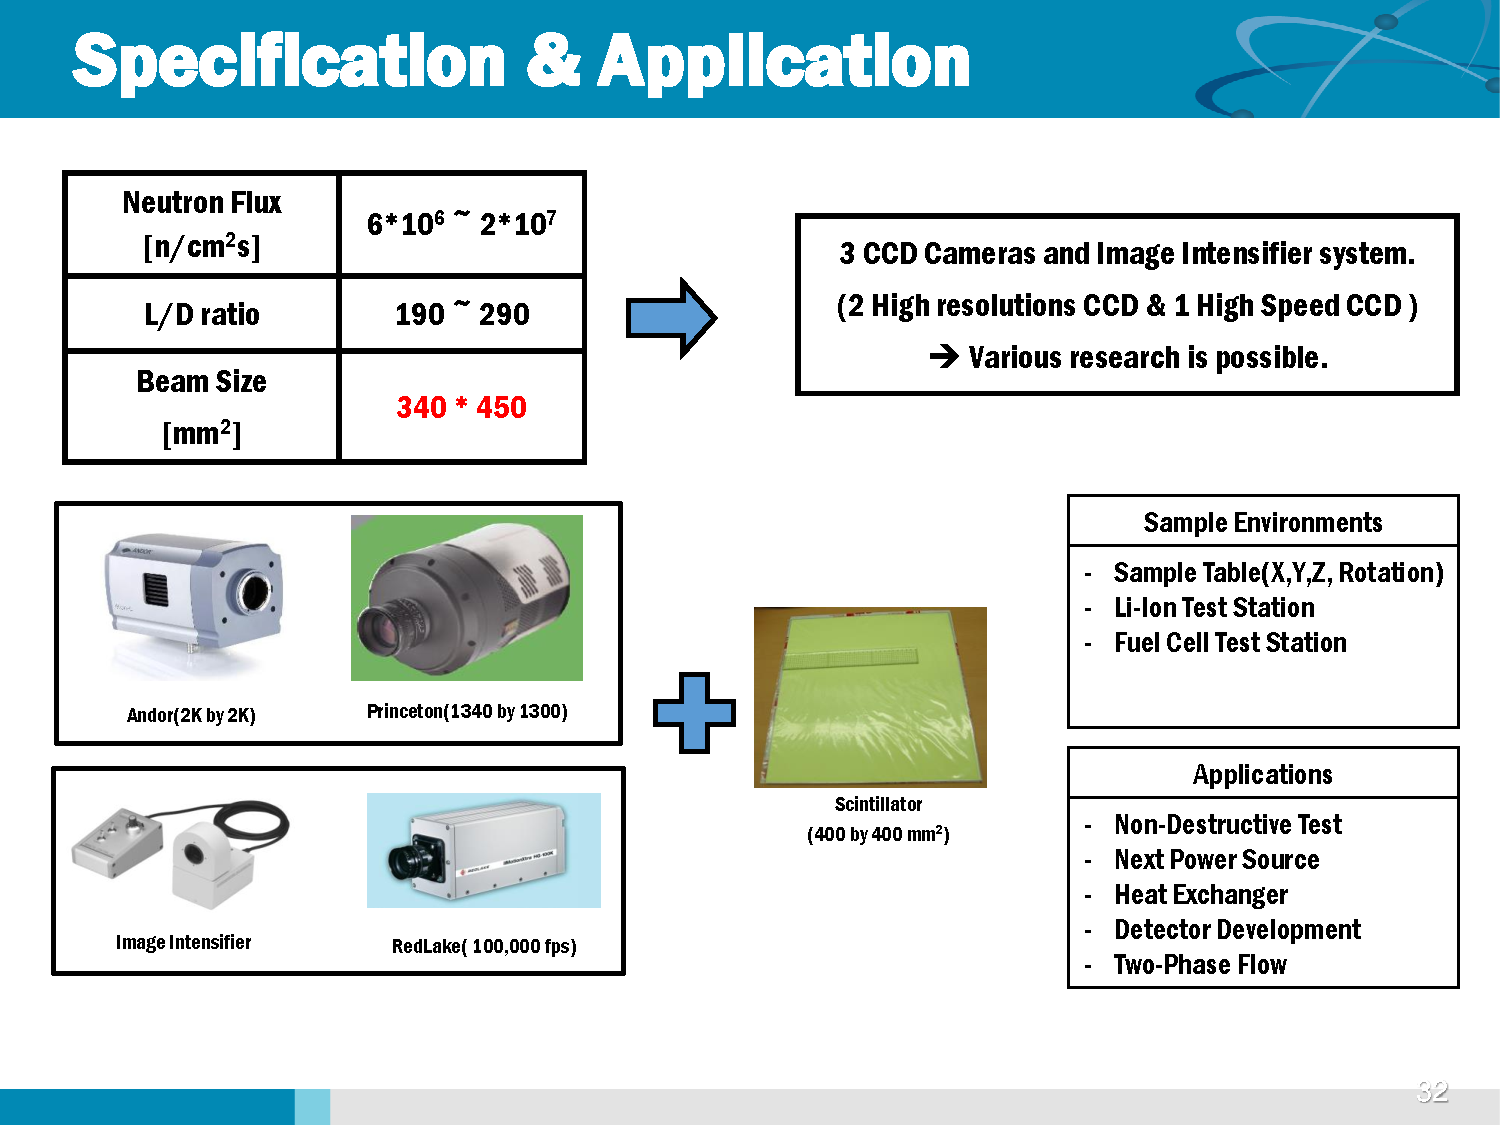
\includepdf{figures/pres2/sl-33.pdf}
\end{frame}

\begin{frame}
  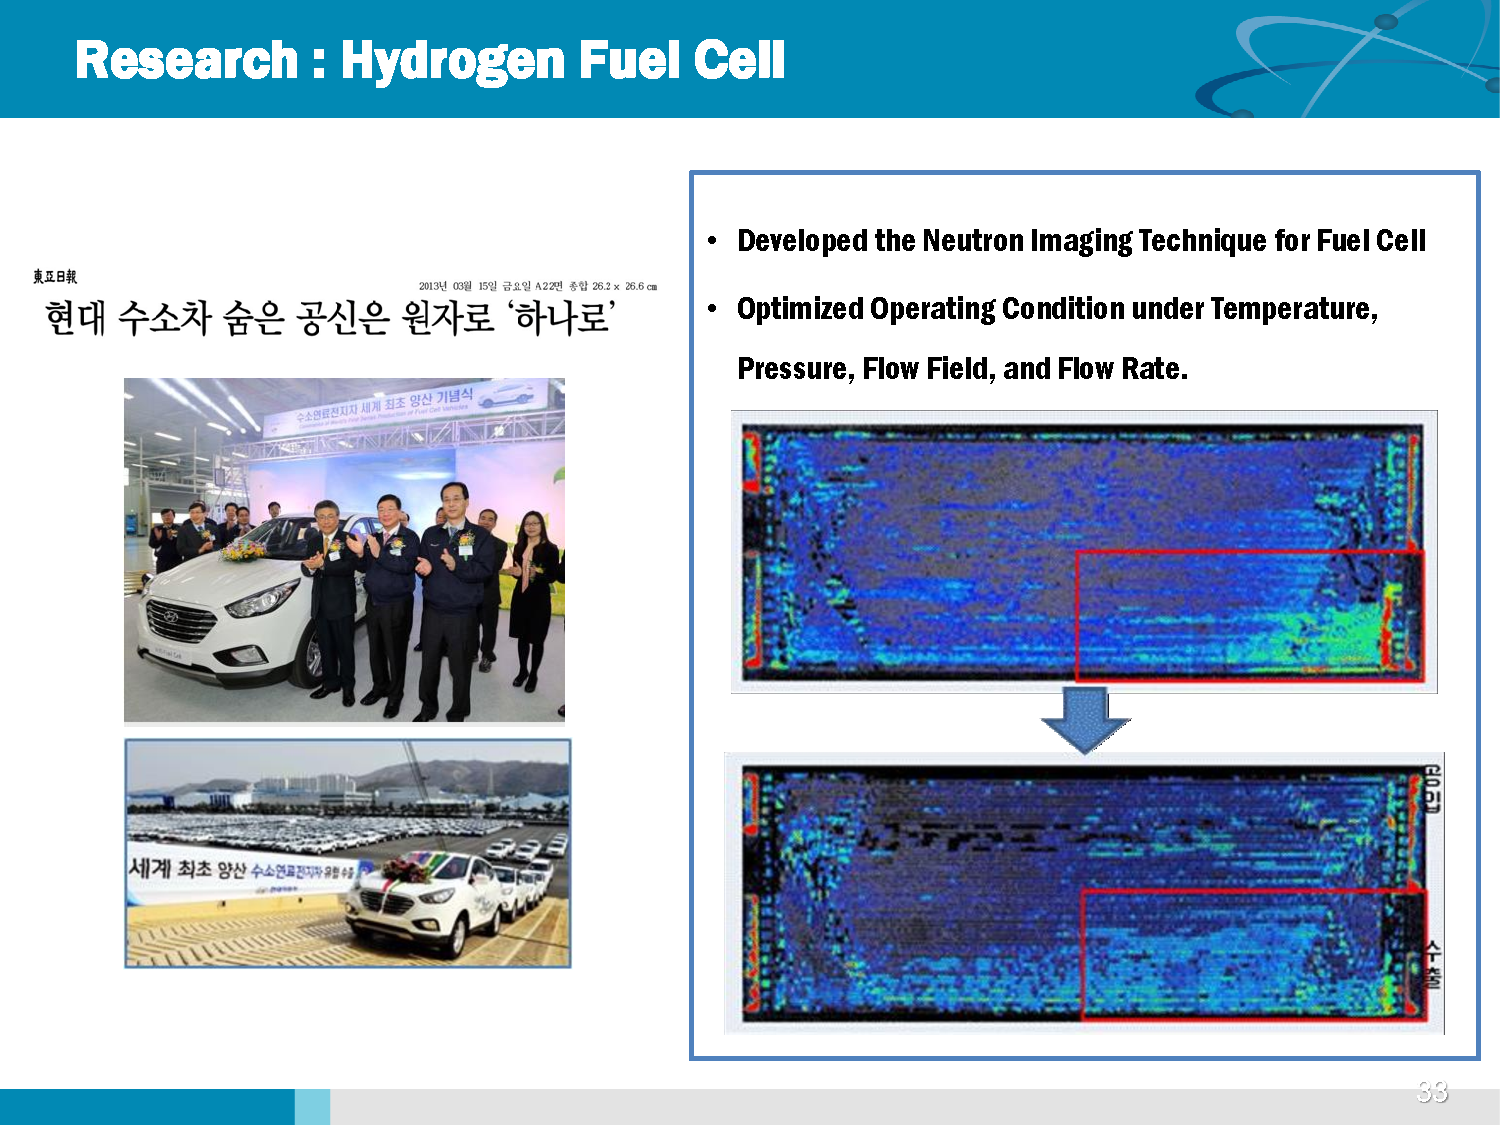
\includepdf{figures/pres2/sl-34.pdf}
\end{frame}

%-------------------------------------------------
\subsection{Instrumentation and Instrument Design for Neutron Imaging}
%-------------------------------------------------
\begin{frame}
  \frametitle{Apresentações escolhidas}
  \framesubtitle{(3)}
  \begin{center}
    Instrumentation and Instrument Design for Neutron Imaging\\
    \vspace{2.0cm}
    N. Kardjilov
  \end{center}
\end{frame}

\begin{frame}
  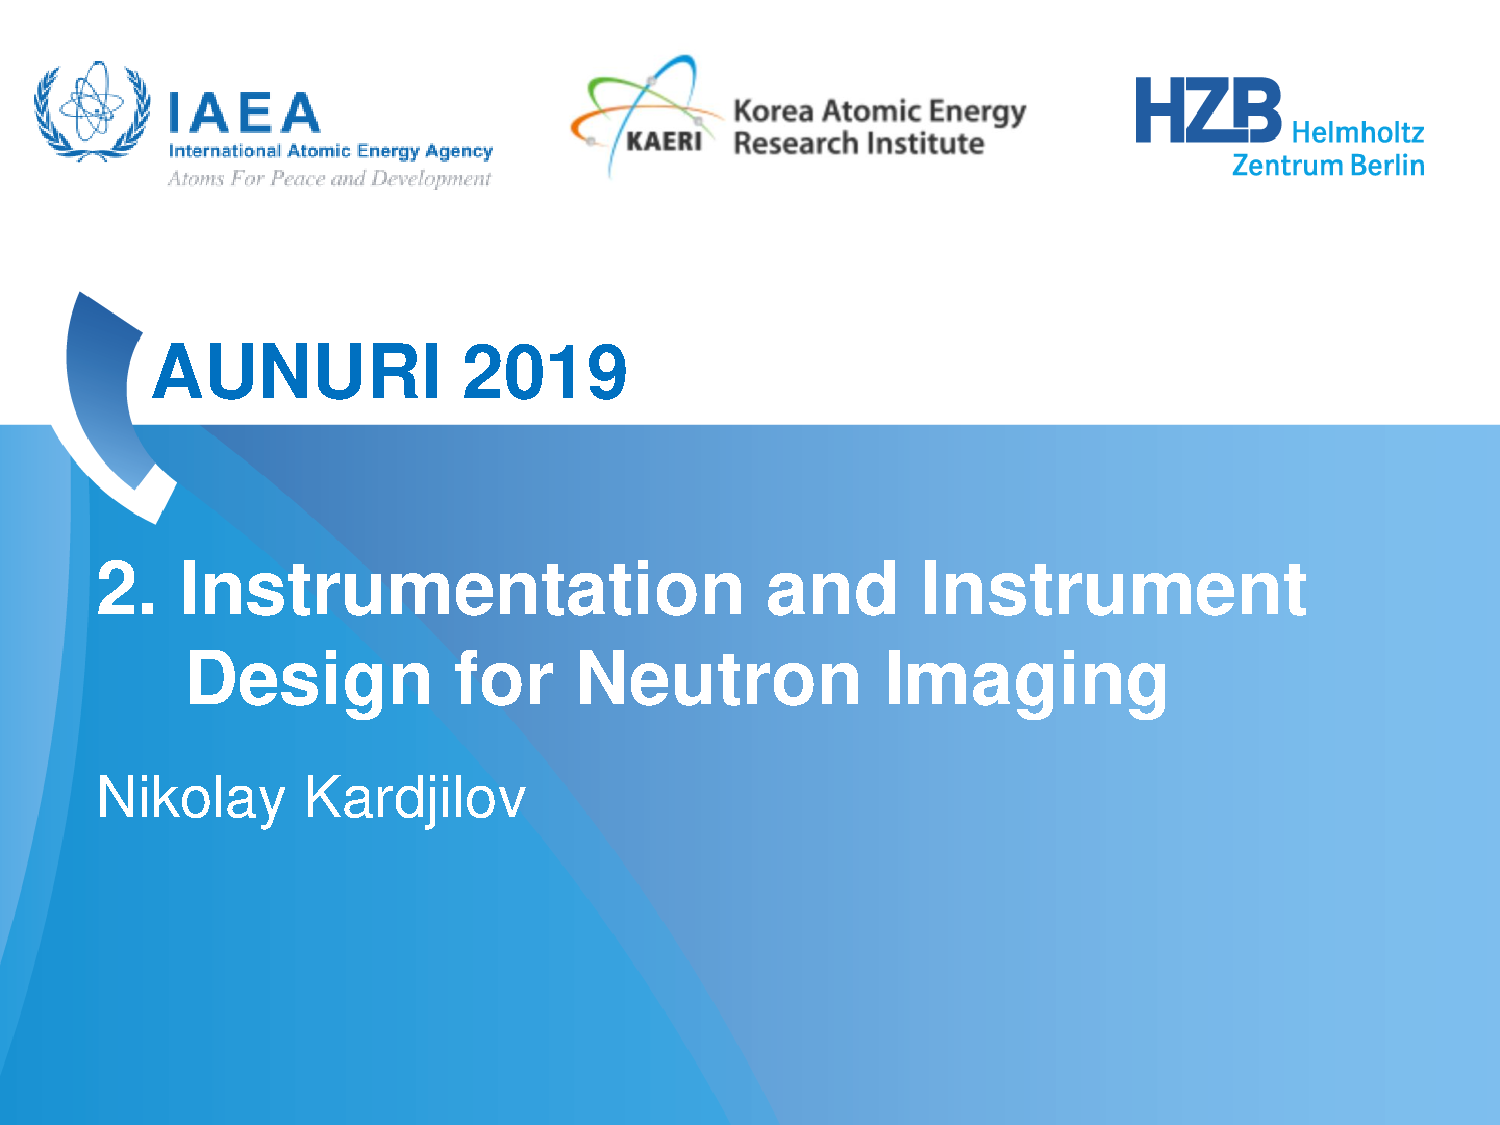
\includepdf{figures/pres3/sl-1.pdf}
\end{frame}

\begin{frame}
  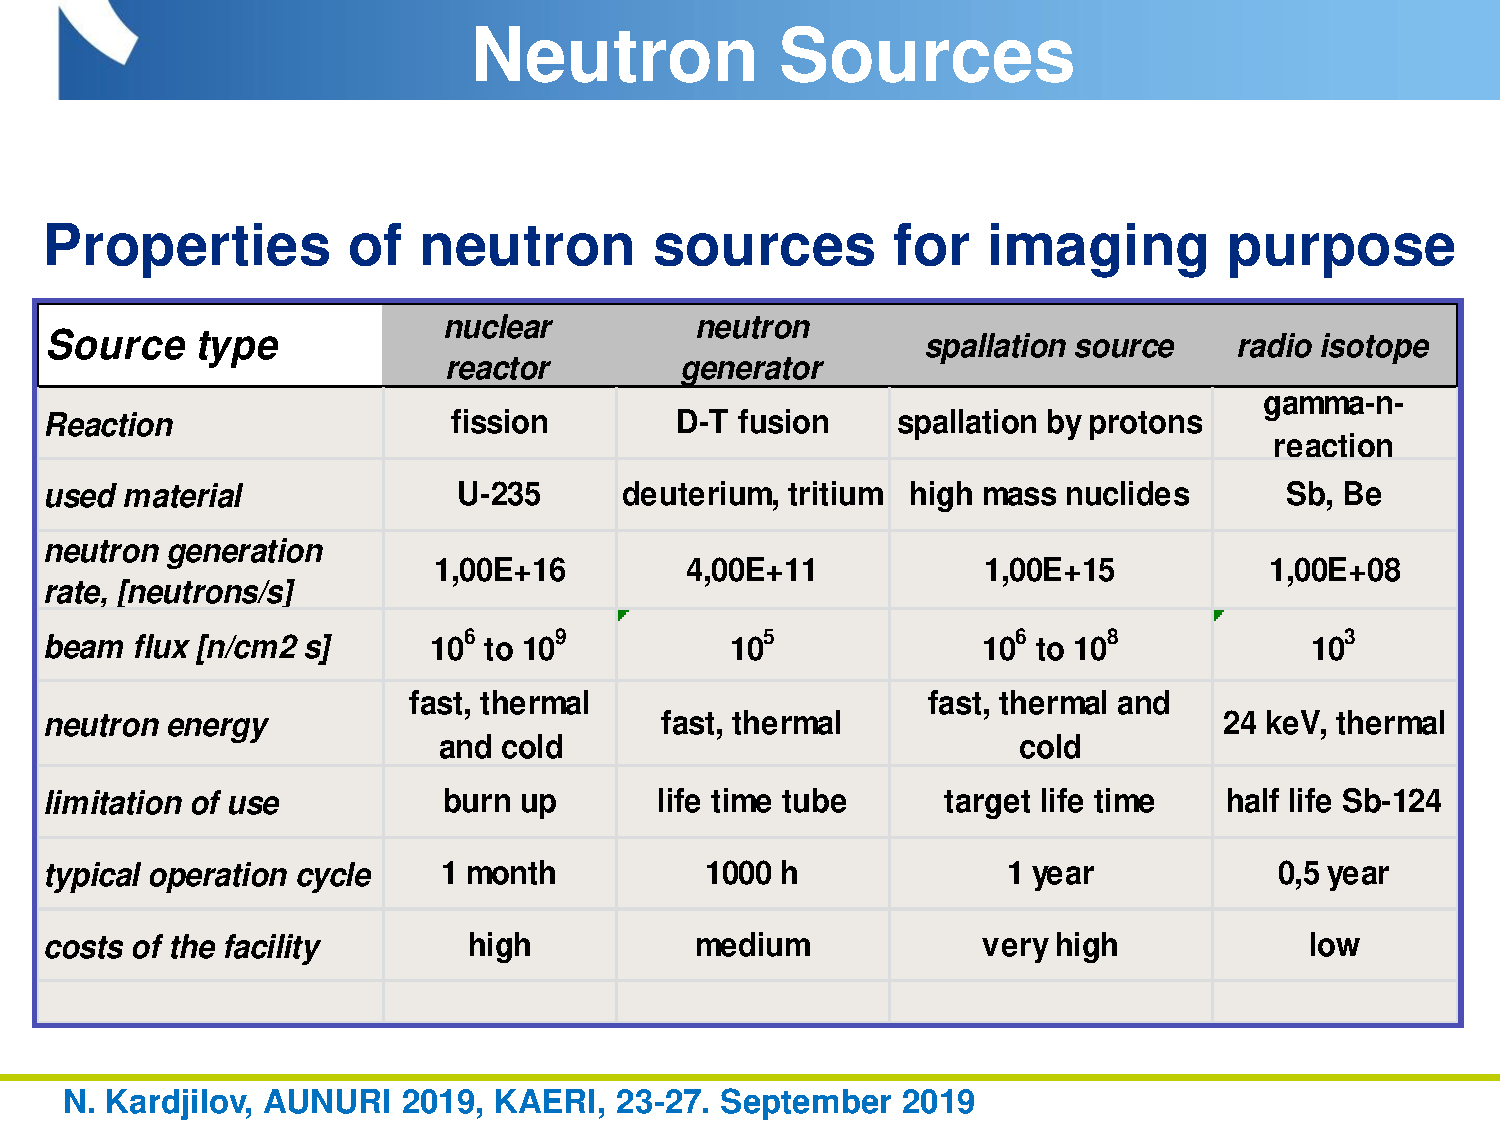
\includepdf{figures/pres3/sl-4.pdf}
\end{frame}
\begin{frame}
  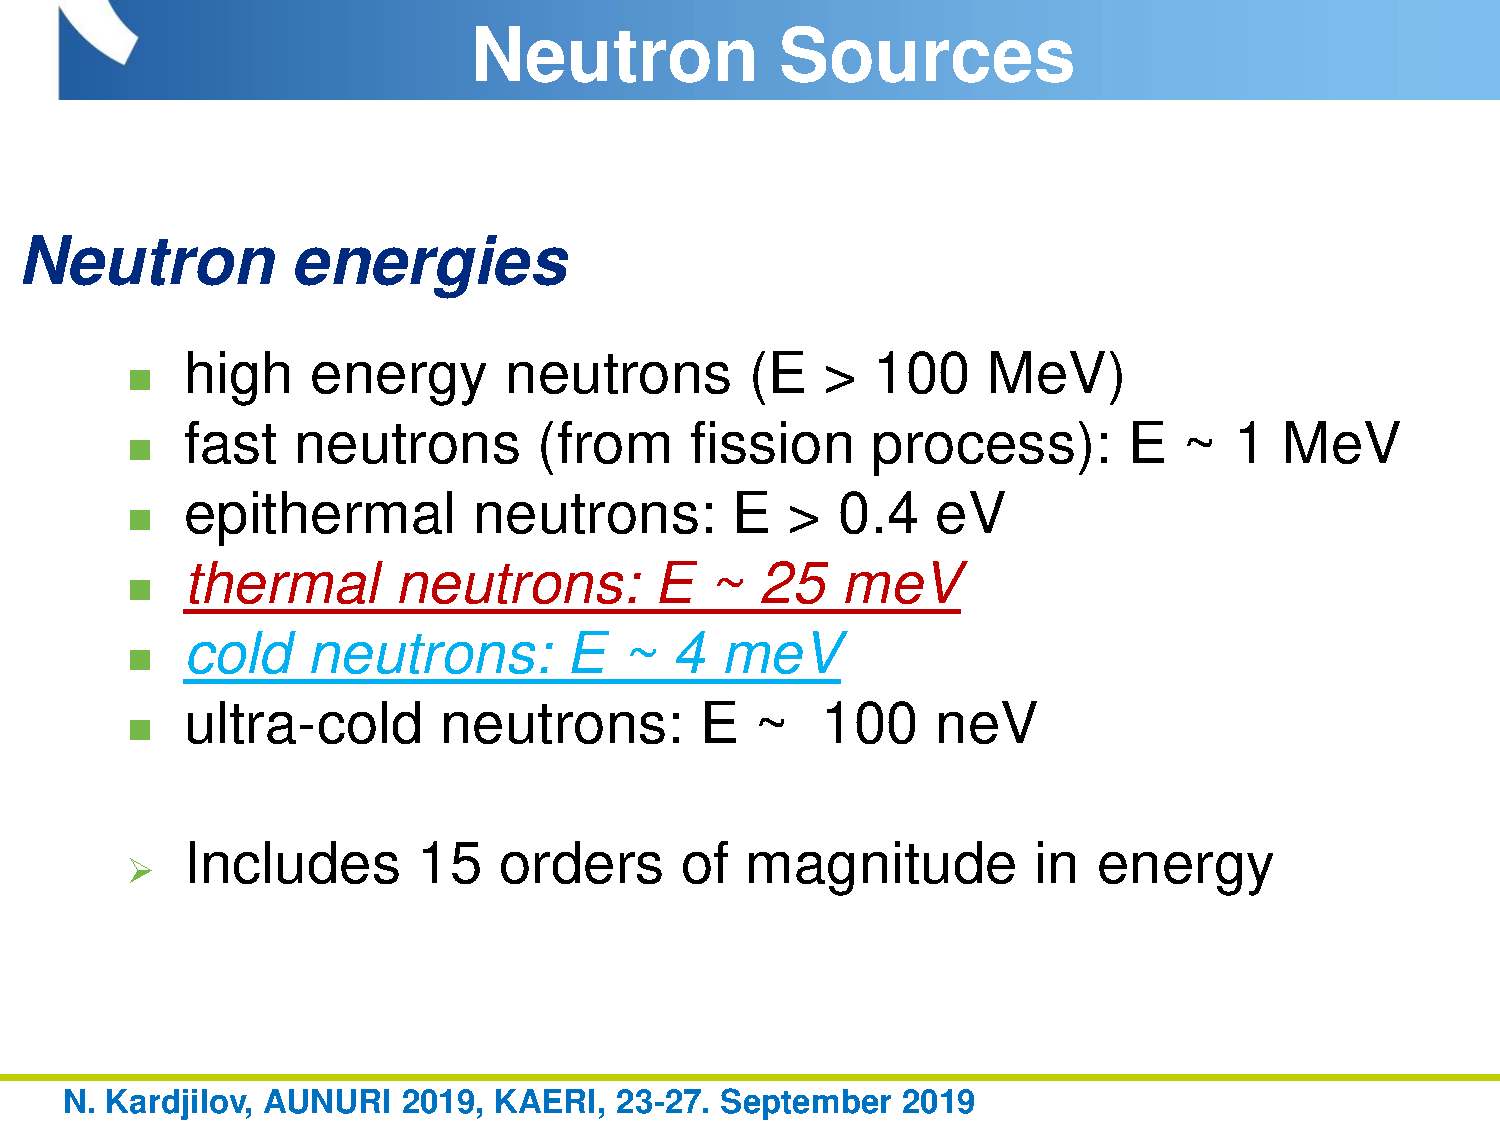
\includepdf{figures/pres3/sl-5.pdf}
\end{frame}
\begin{frame}
  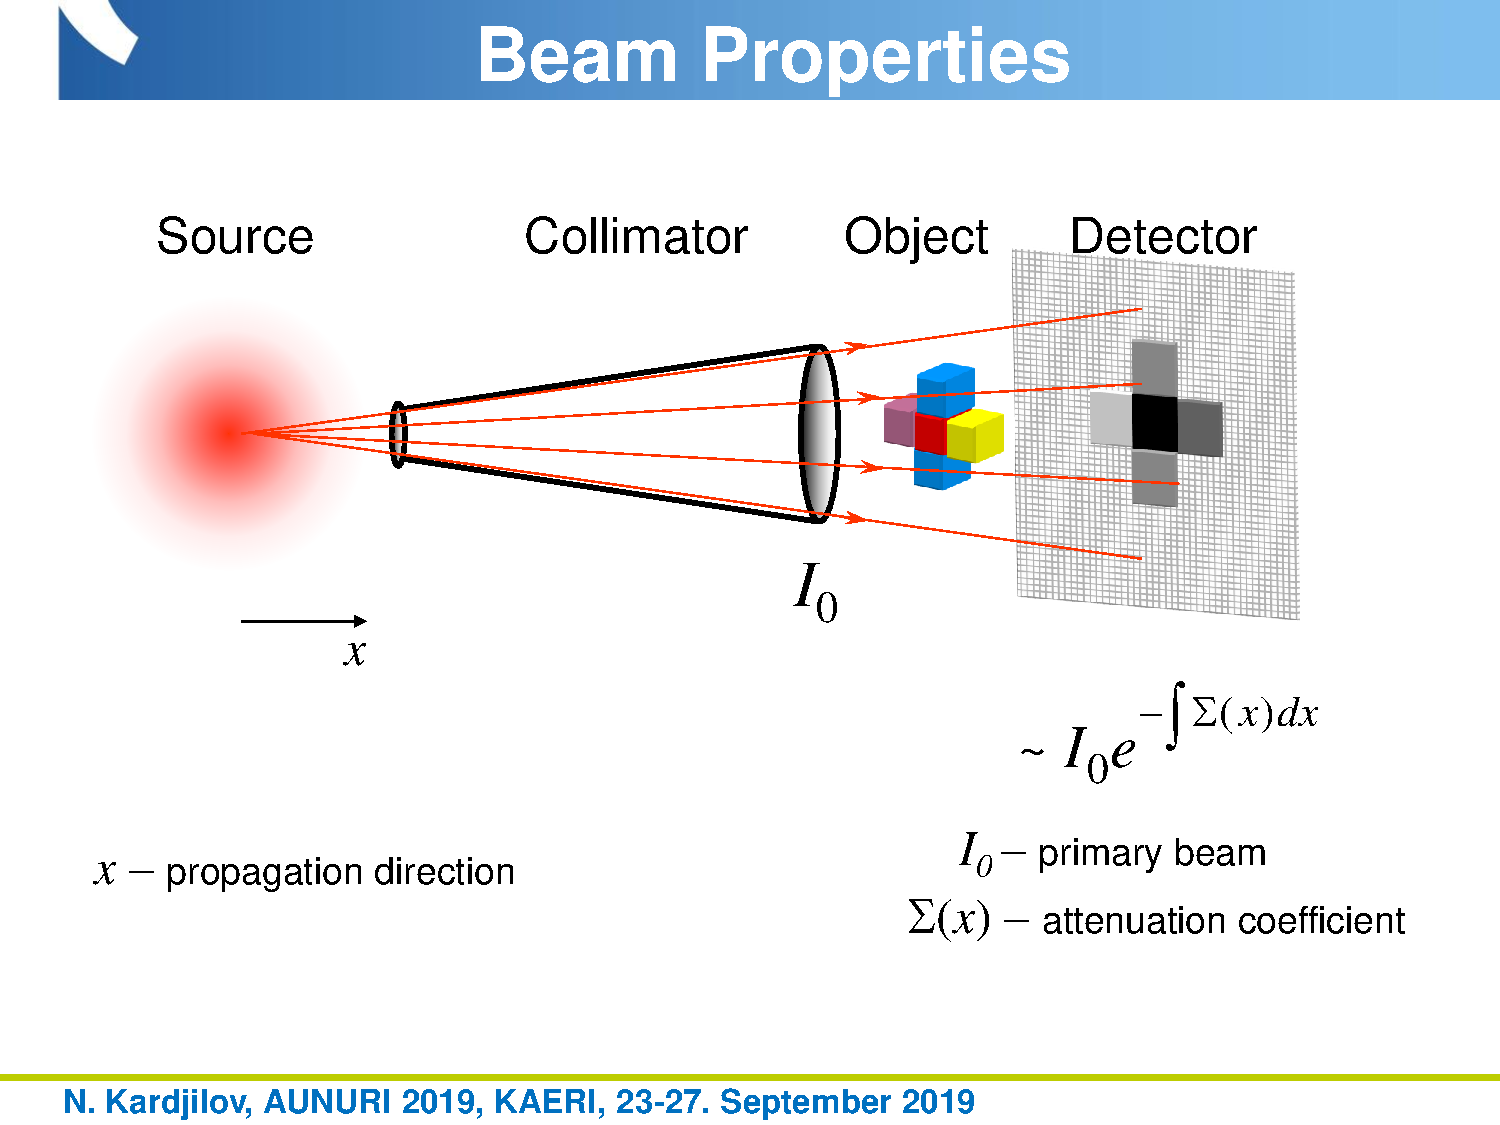
\includepdf{figures/pres3/sl-14.pdf}
\end{frame}
\begin{frame}
  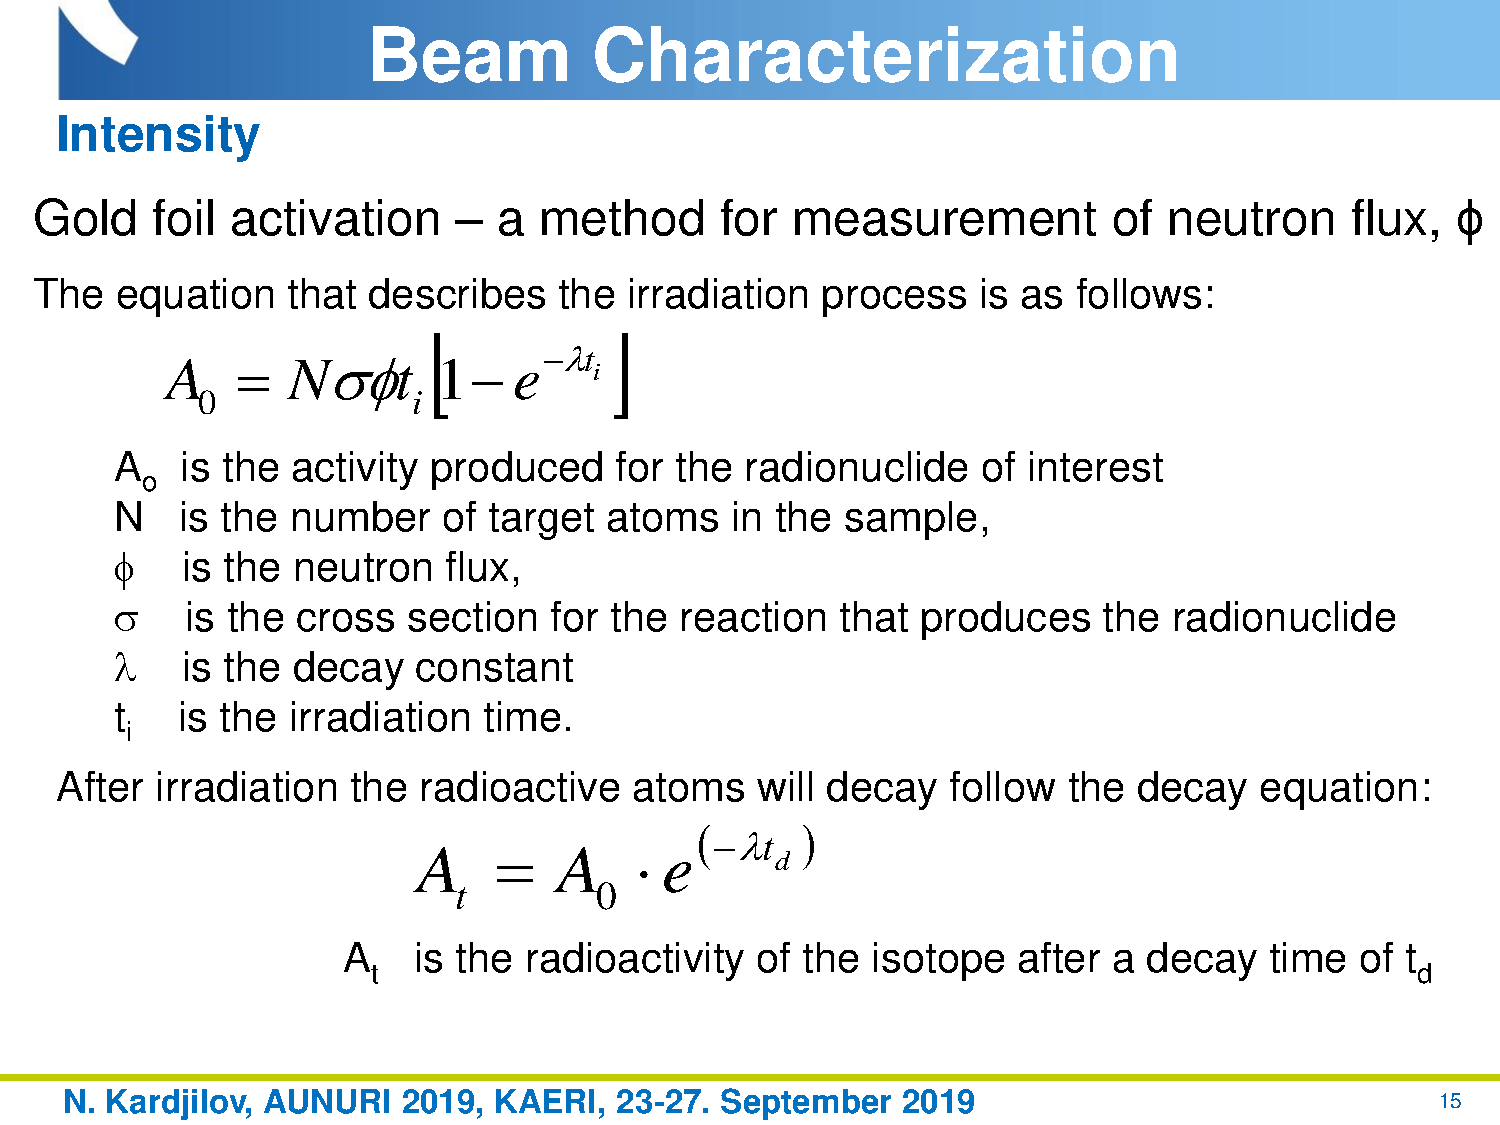
\includepdf{figures/pres3/sl-15.pdf}
\end{frame}
\begin{frame}
  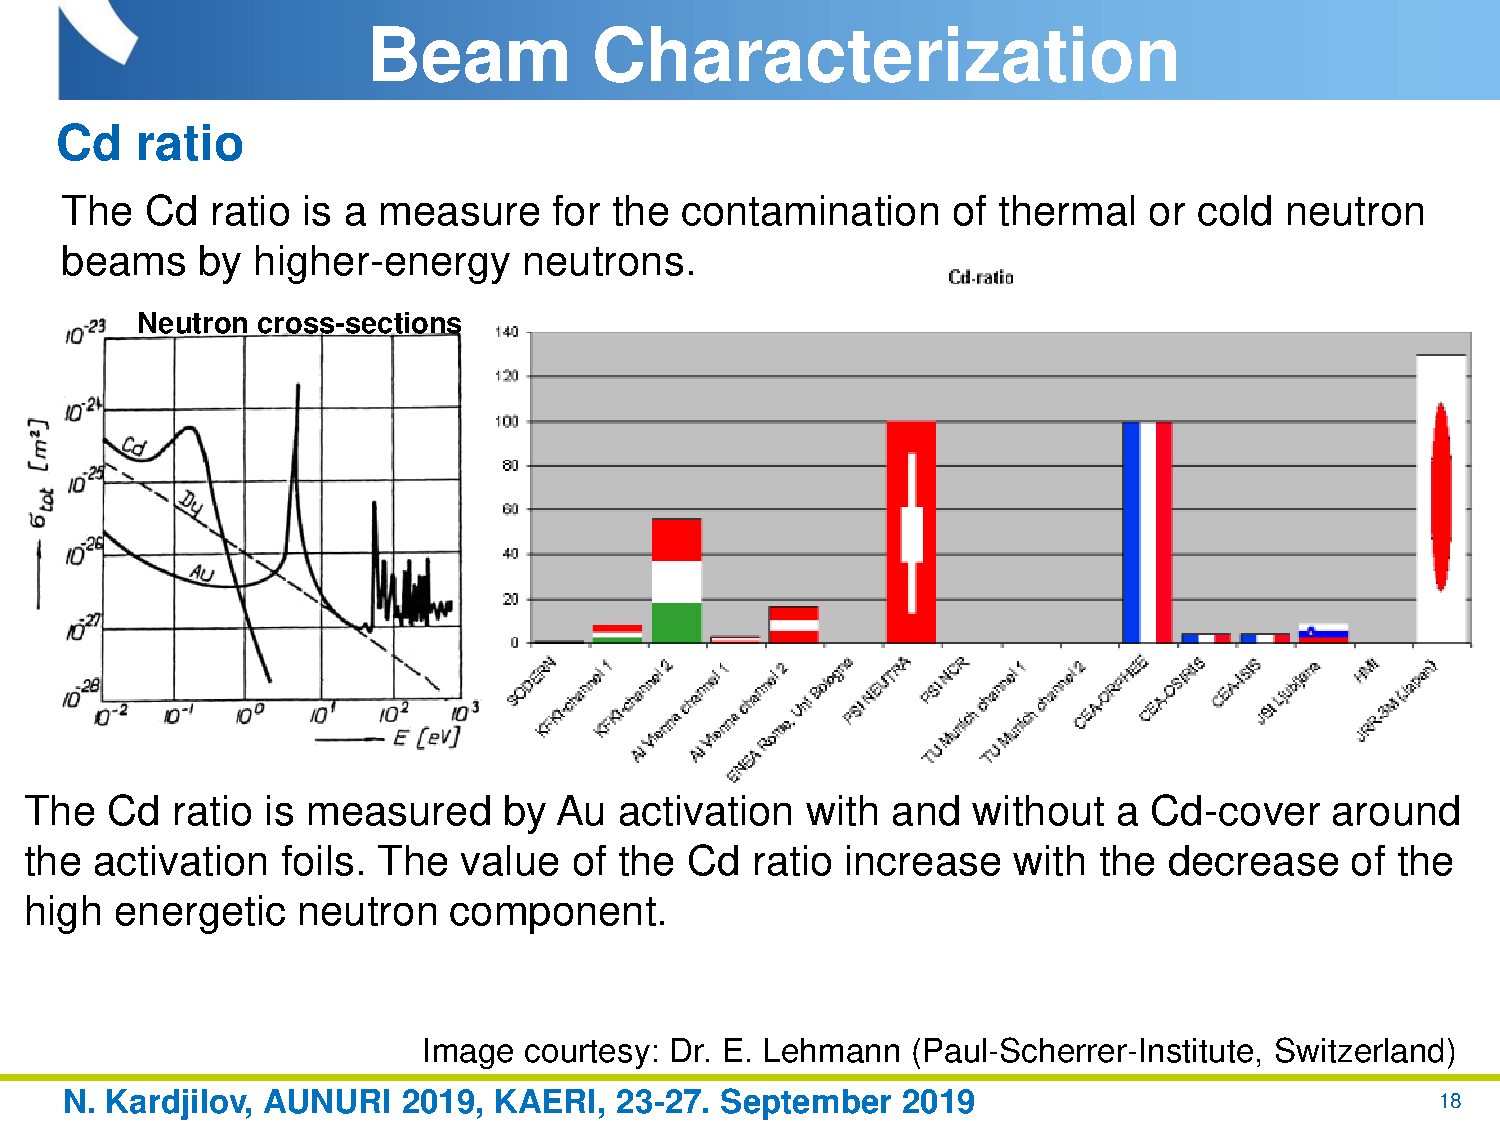
\includepdf{figures/pres3/sl-18.pdf}
\end{frame}
\begin{frame}
  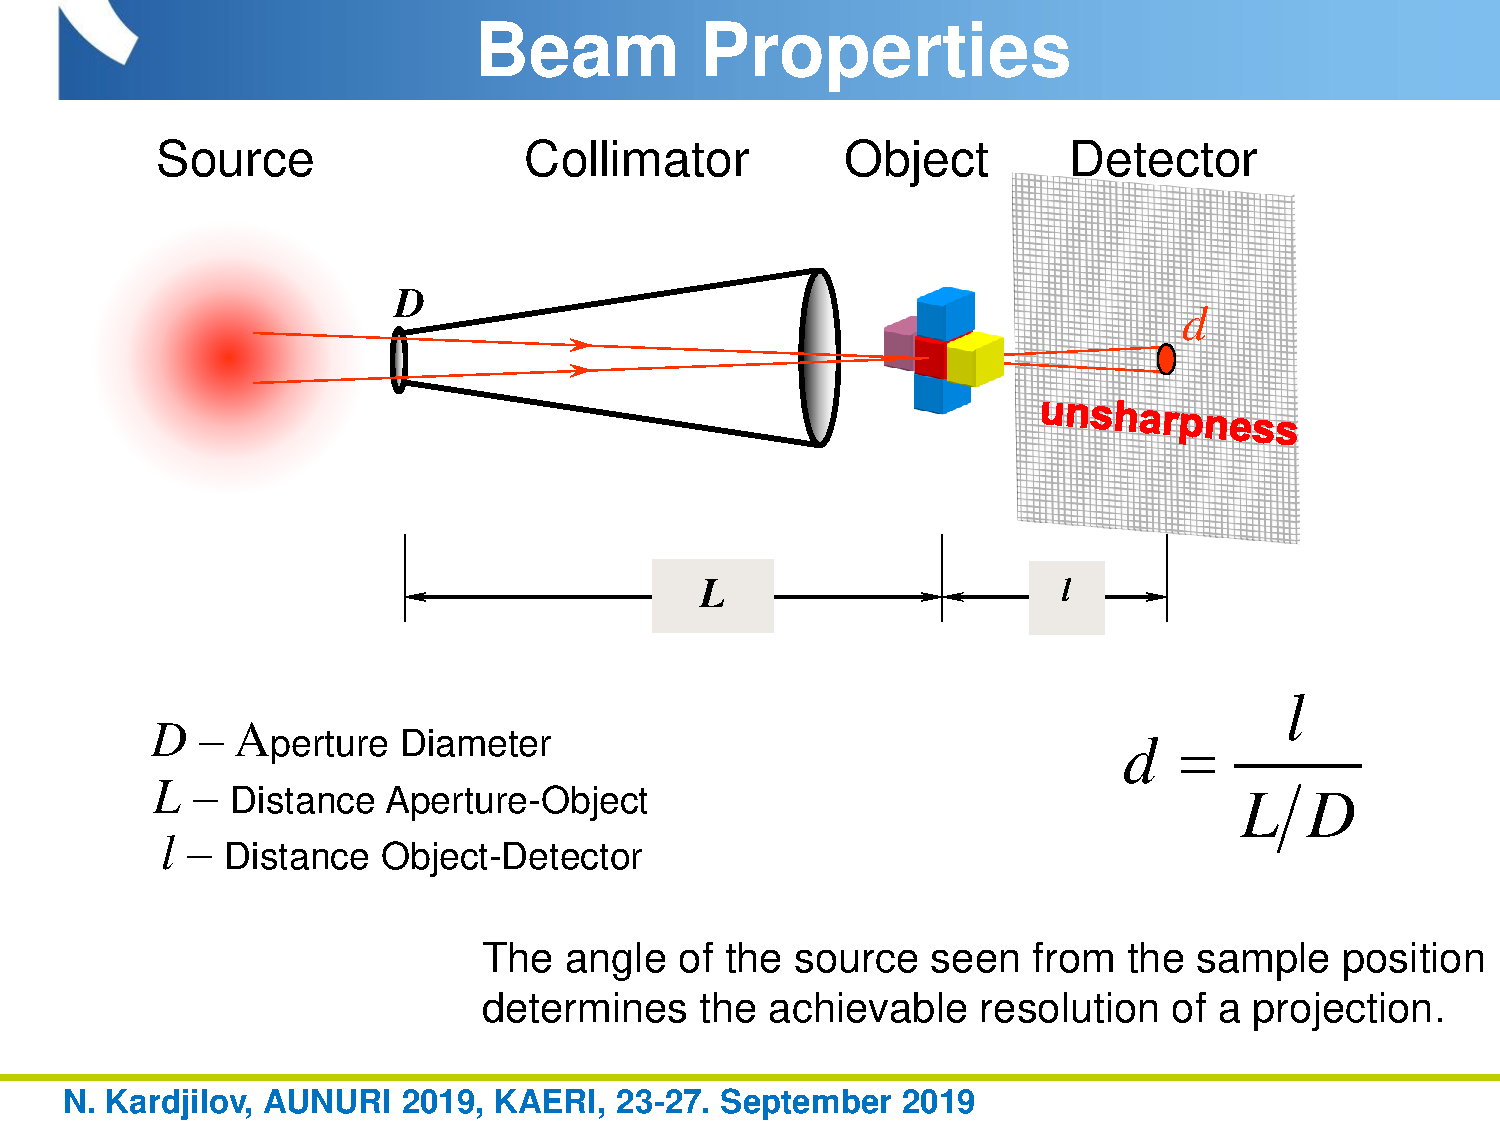
\includepdf{figures/pres3/sl-19.pdf}
\end{frame}
\begin{frame}
  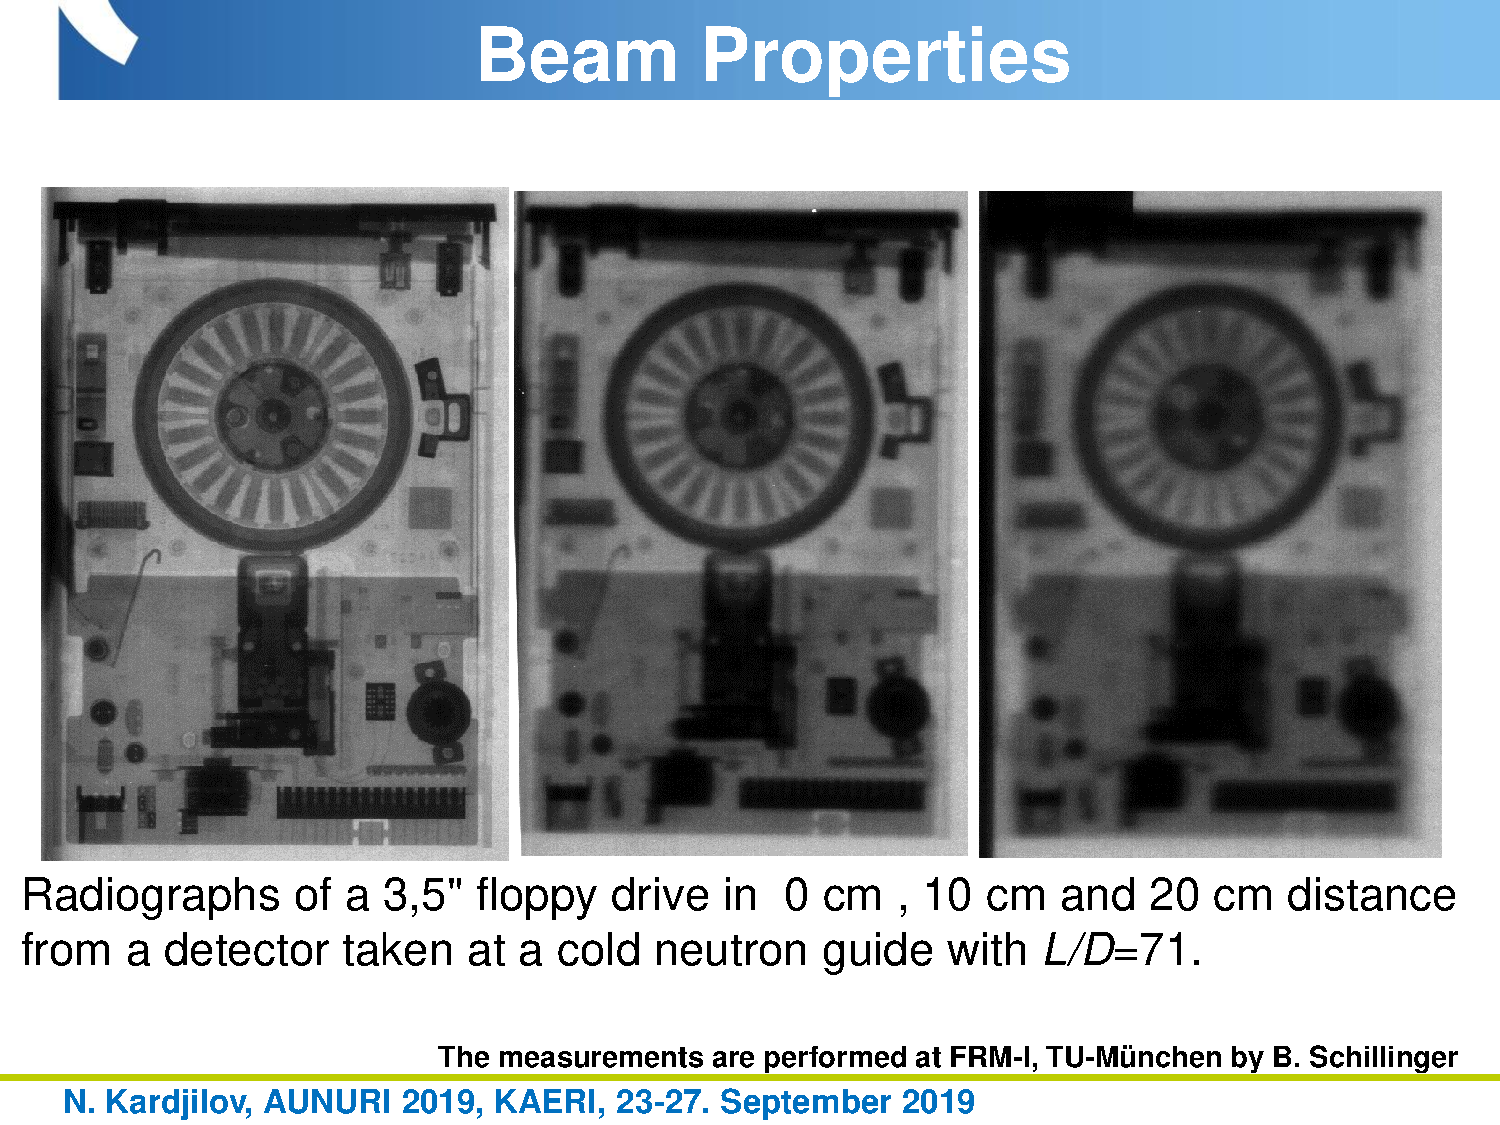
\includepdf{figures/pres3/sl-20.pdf}
\end{frame}
\begin{frame}
  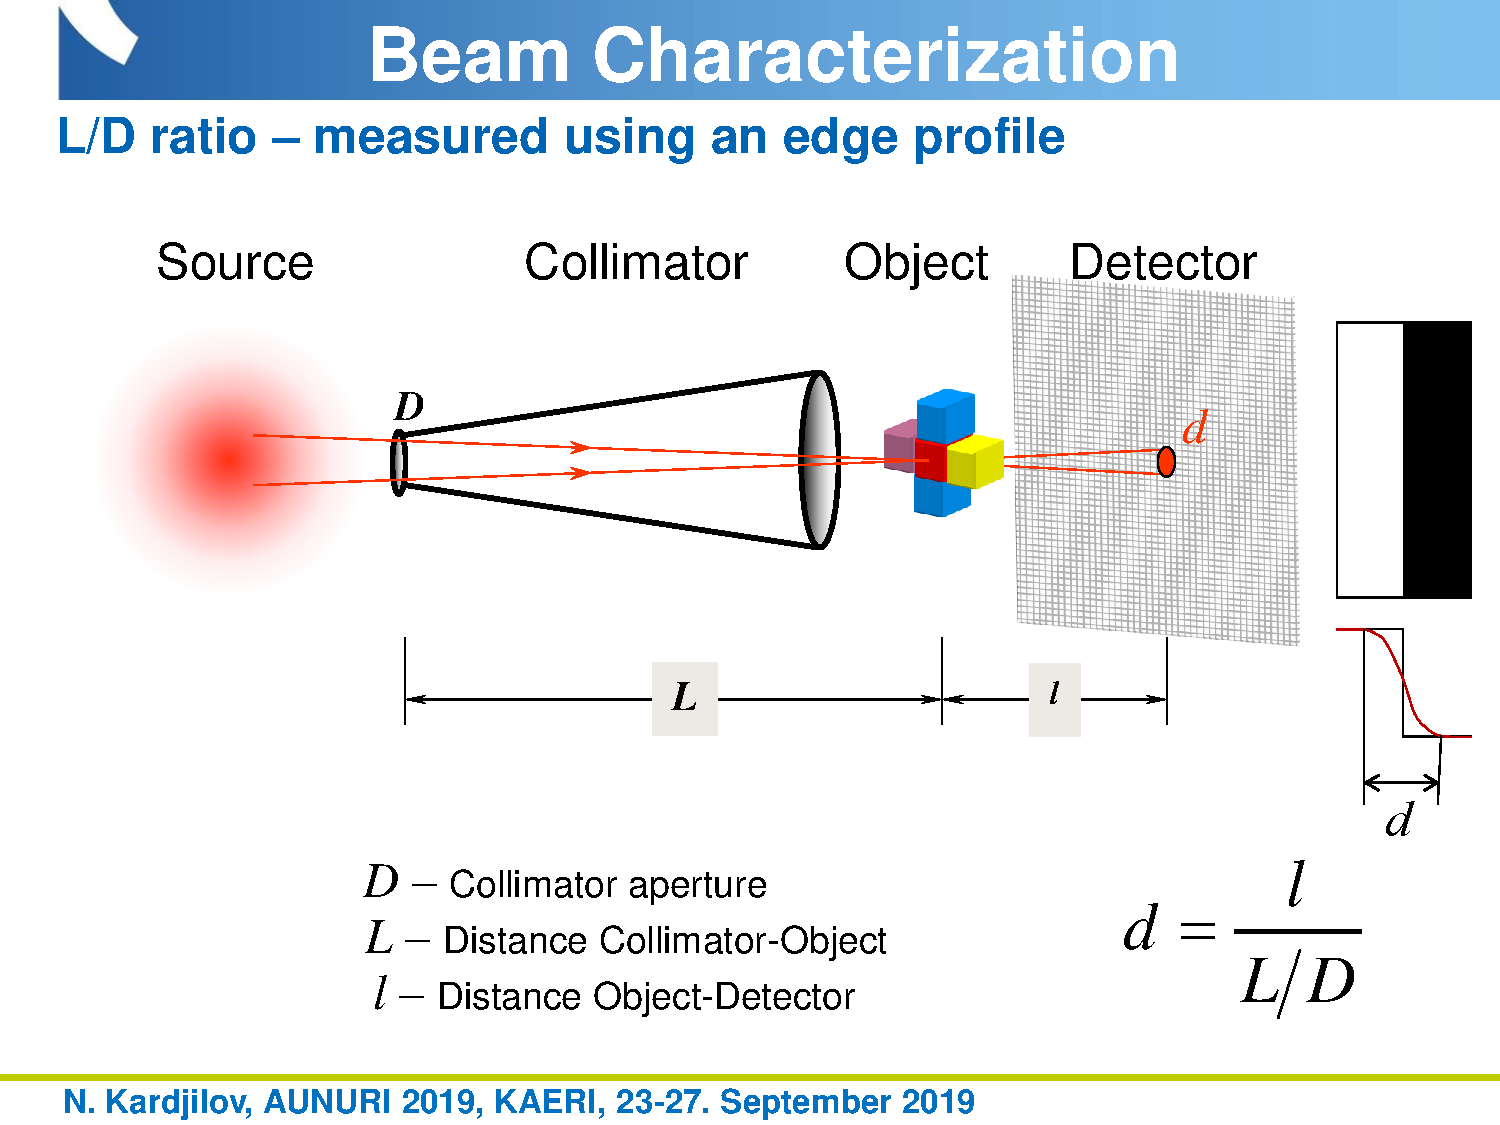
\includepdf{figures/pres3/sl-22.pdf}
\end{frame}
\begin{frame}
  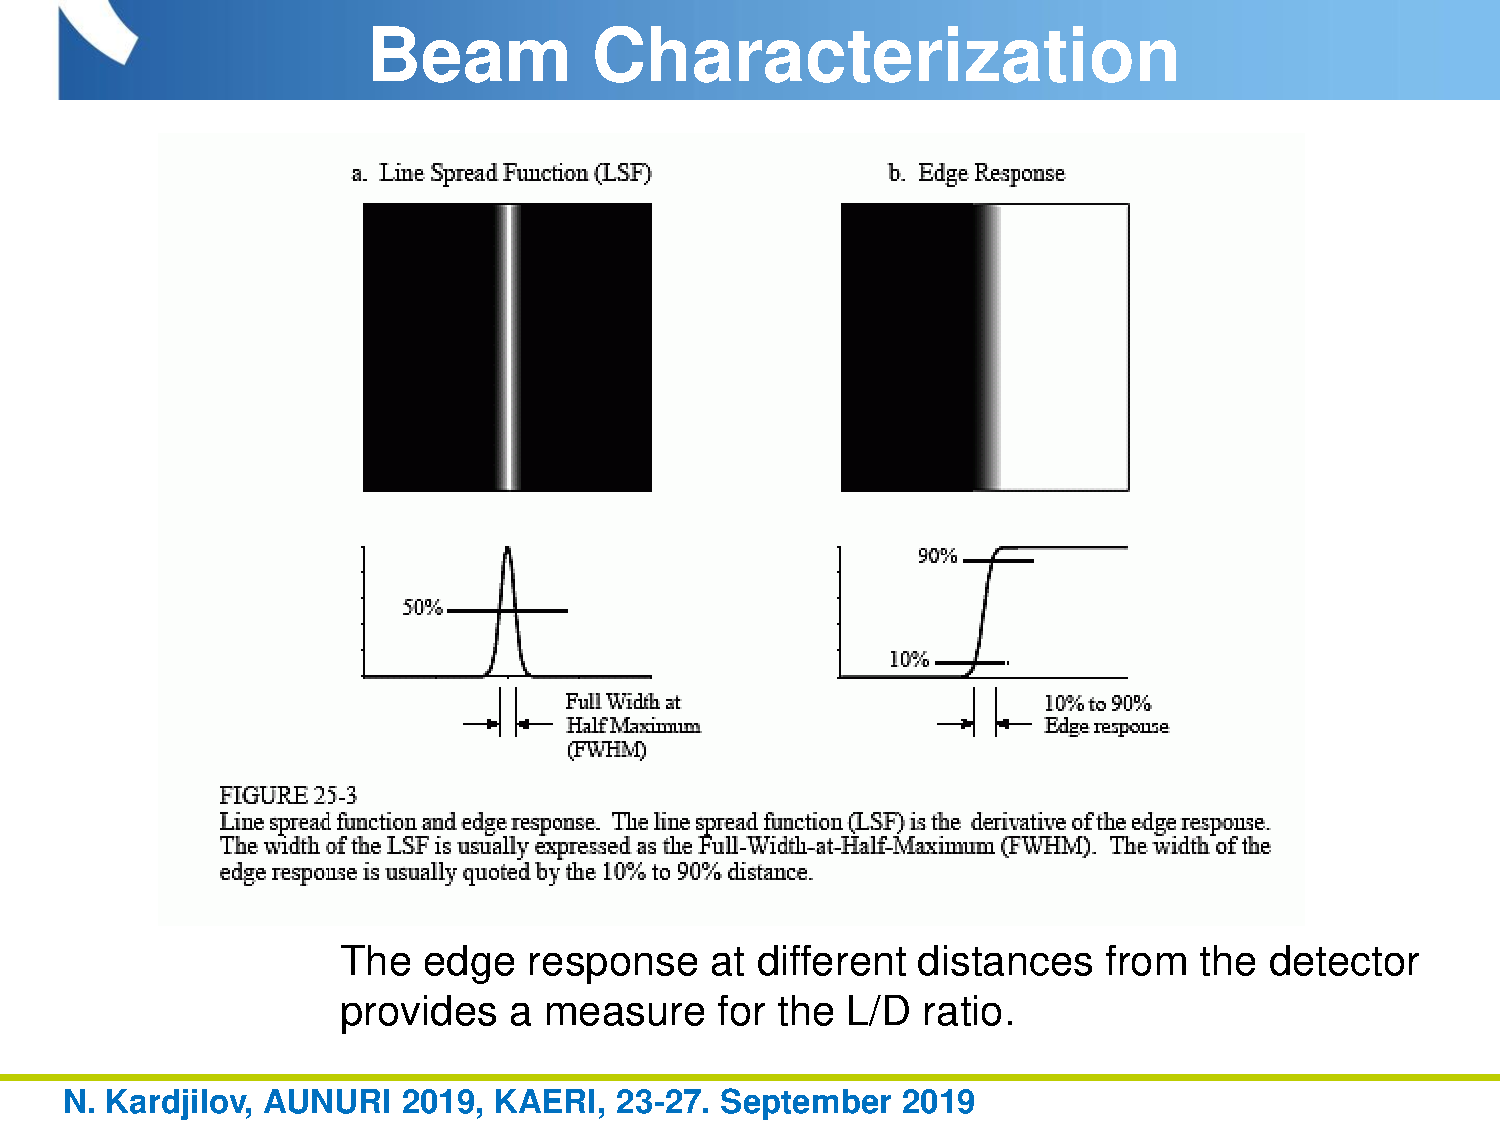
\includepdf{figures/pres3/sl-23.pdf}
\end{frame}
\begin{frame}
  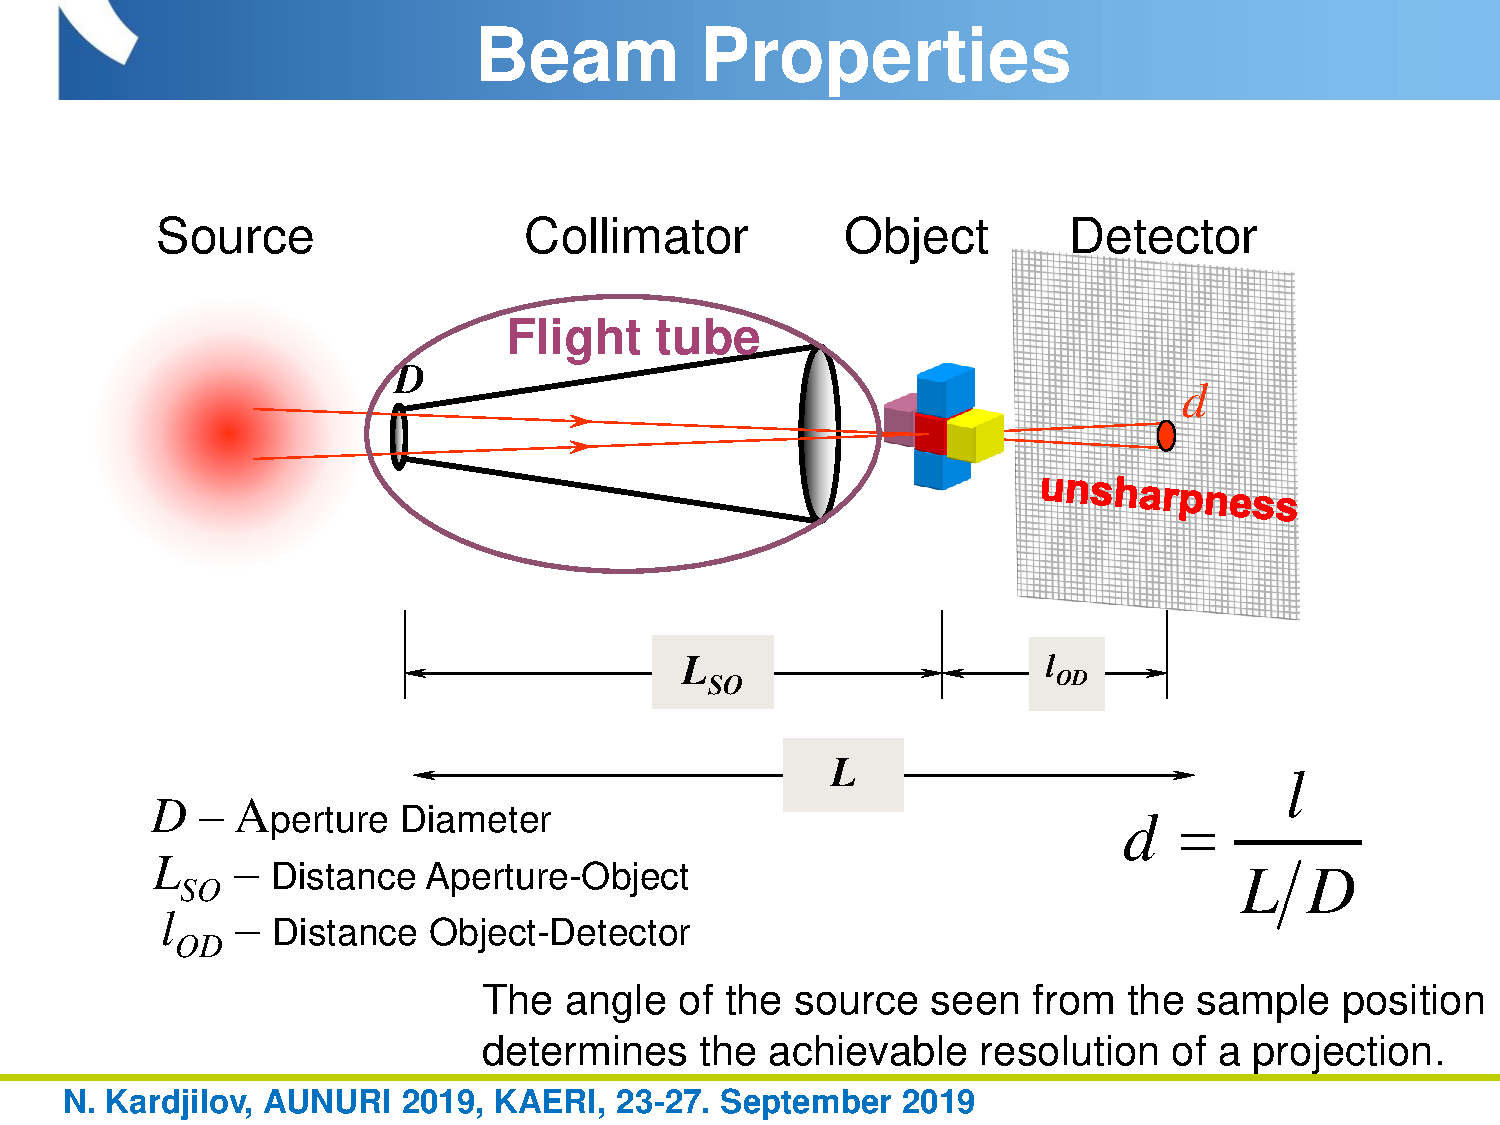
\includepdf{figures/pres3/sl-25.pdf}
\end{frame}
\begin{frame}
  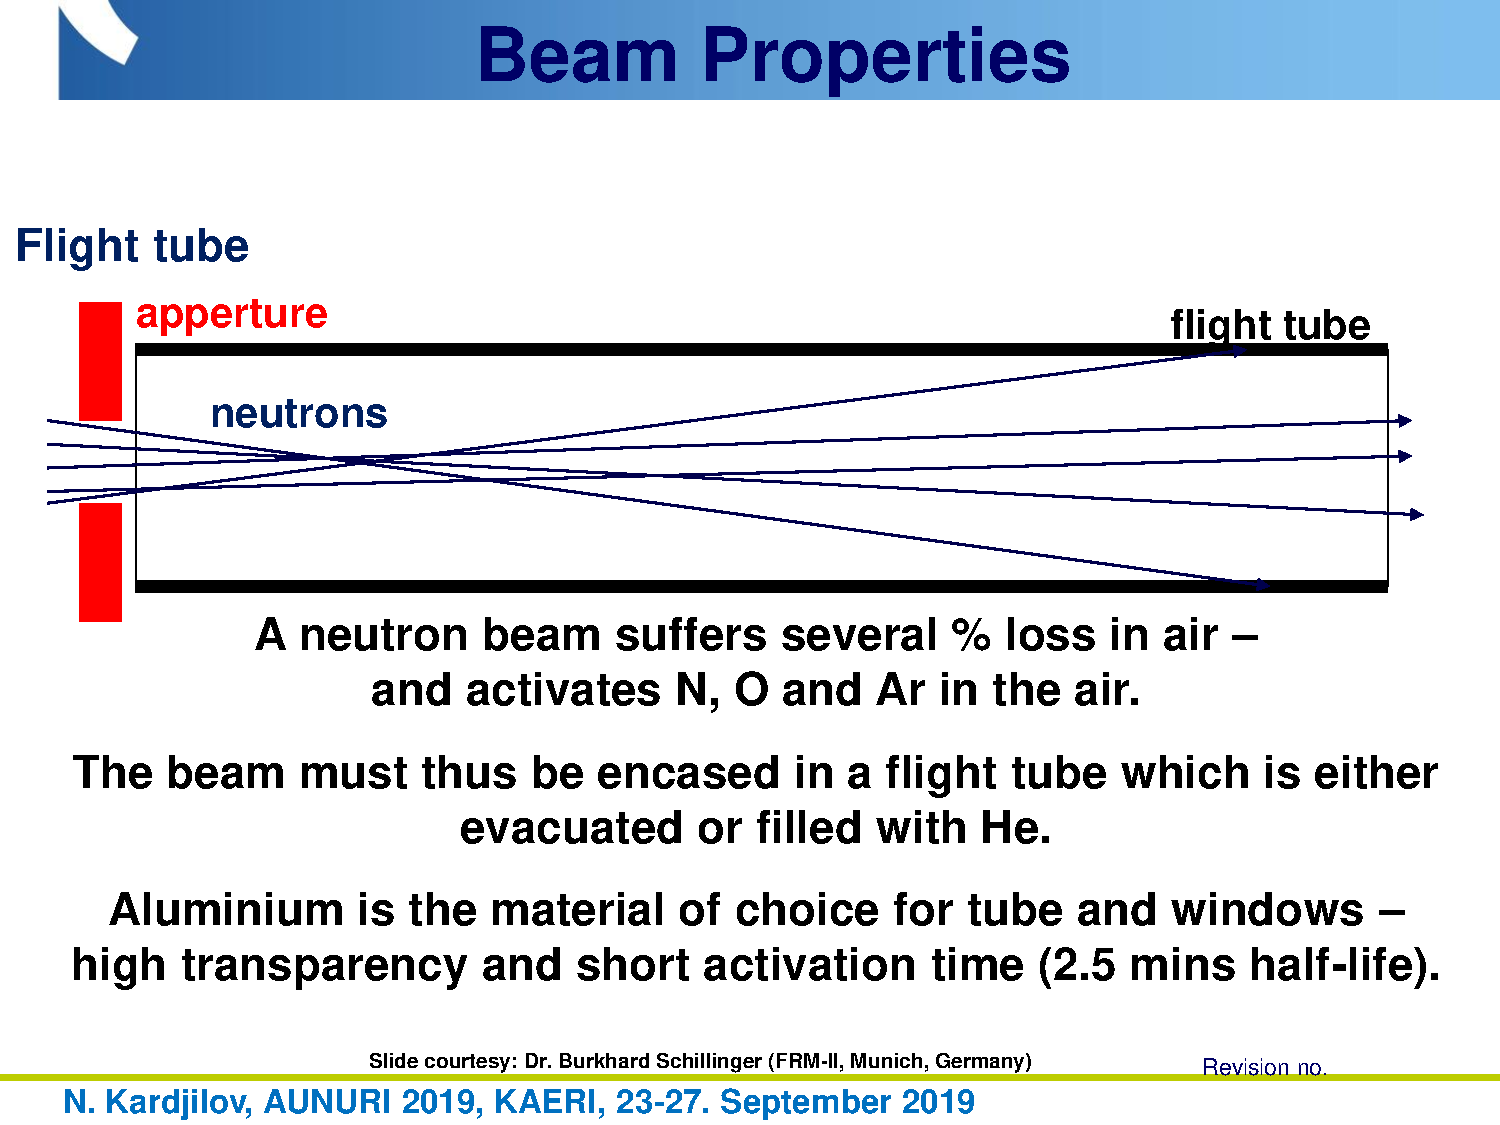
\includepdf{figures/pres3/sl-26.pdf}
\end{frame}
\begin{frame}
  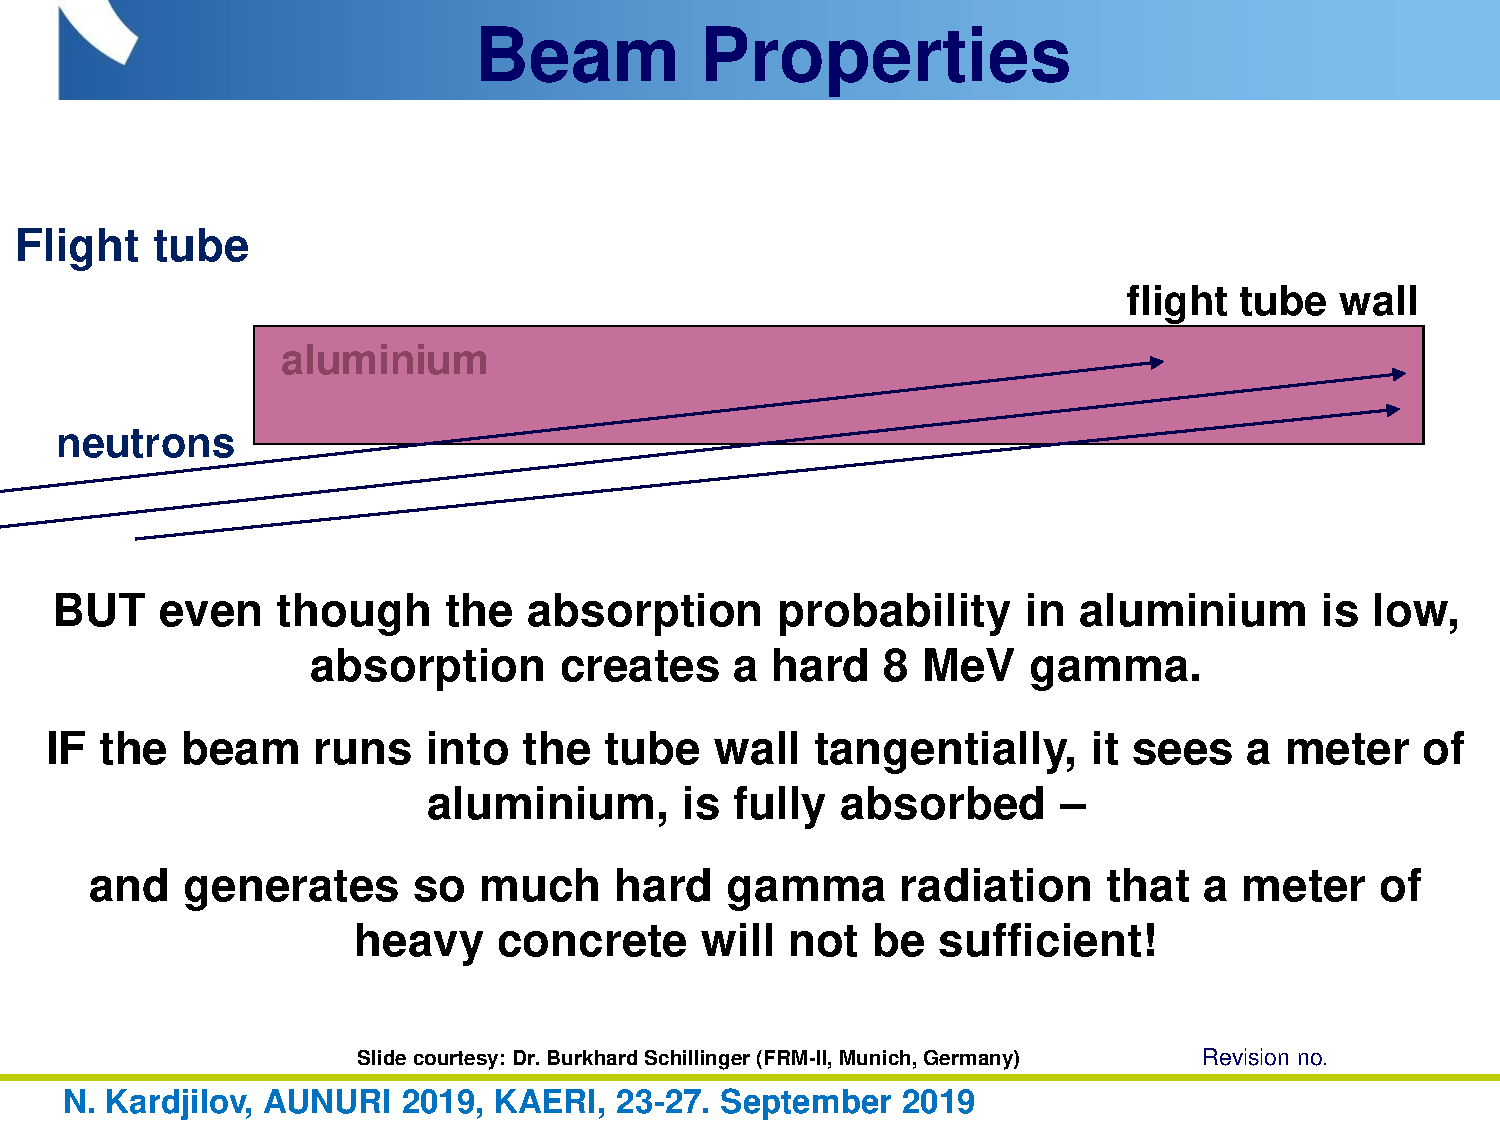
\includepdf{figures/pres3/sl-27.pdf}
\end{frame}
\begin{frame}
  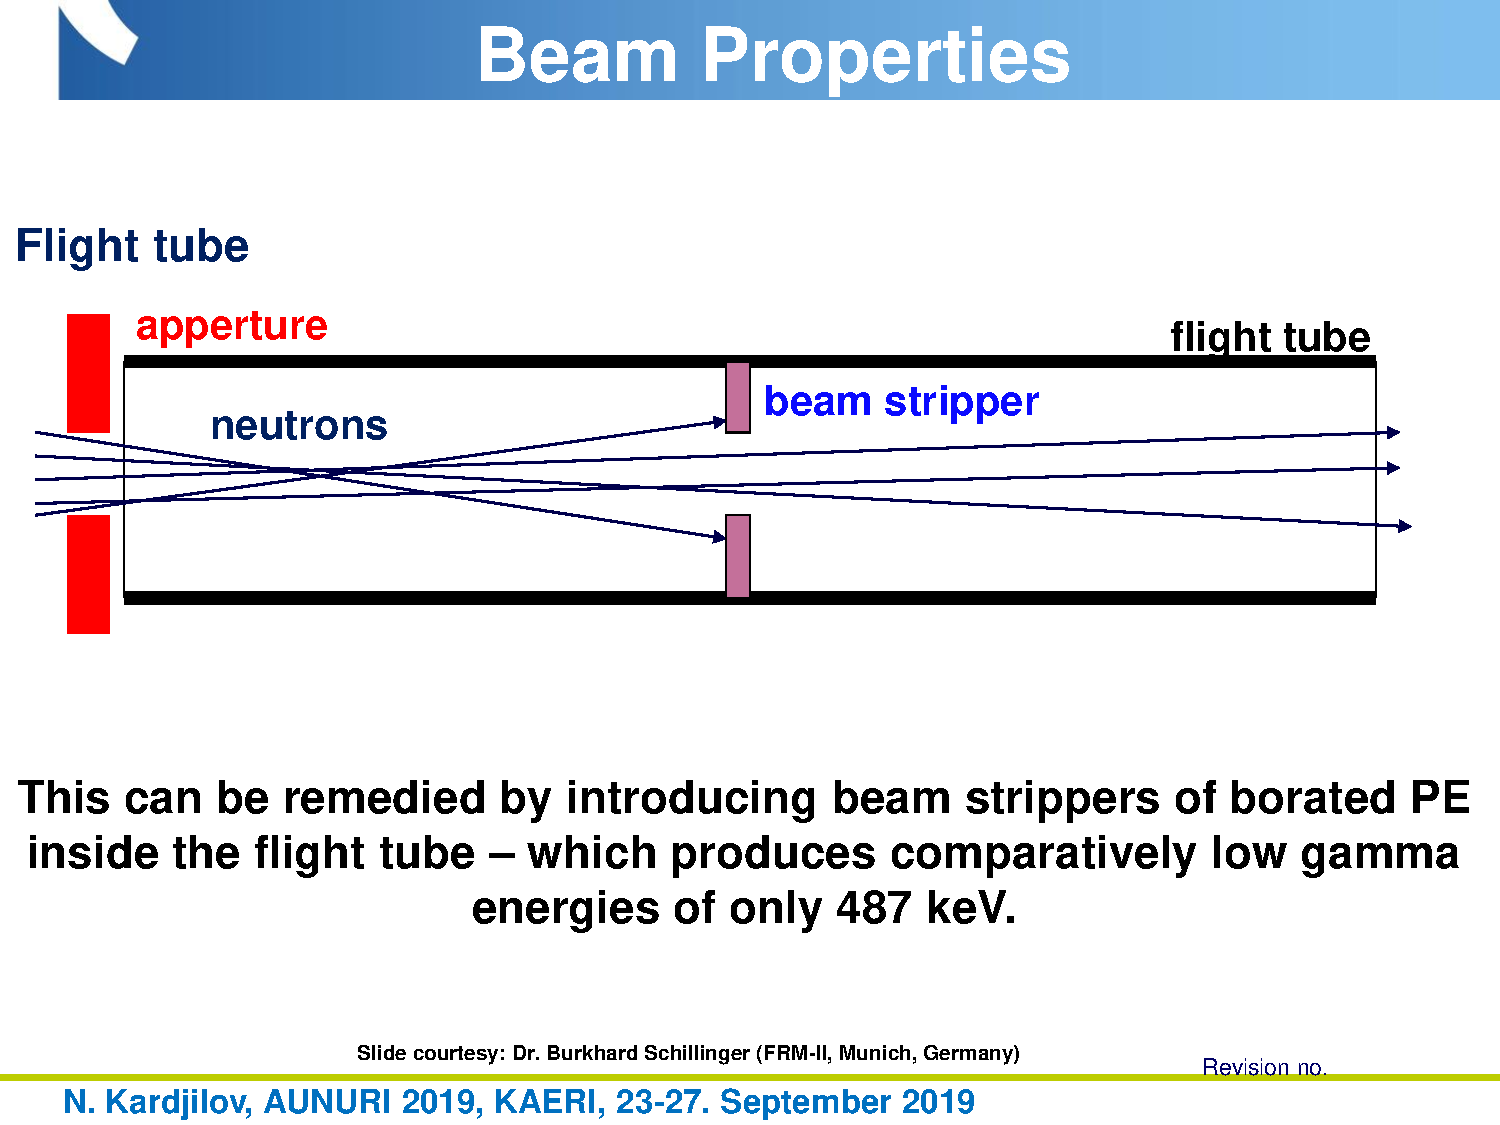
\includepdf{figures/pres3/sl-28.pdf}
\end{frame}

%-------------------------------------------------
\subsection{Detectors for Neutron Imaging}
%-------------------------------------------------
\begin{frame}
  \frametitle{Apresentações escolhidas}
  \framesubtitle{(4)}
  \begin{center}
    Detectors for Neutron Imaging\\
    \vspace{2.0cm}
    N. Kardjilov
  \end{center}
\end{frame}

%-------------------------------------------------
\subsection{Simulation of Neutron Imaging Experiments using McStats and MCNP software tools}
%-------------------------------------------------
\begin{frame}
  \frametitle{Apresentações escolhidas}
  \framesubtitle{(5)}
  \begin{center}
    Simulation of Neutron Imaging Experiments using McStats and MCNP software tools\\
    \vspace{2.0cm}
    N. Kardjilov
  \end{center}
\end{frame}

%-------------------------------------------------
\subsection{The IAEA Neutron Imaging e-learning course project}
%-------------------------------------------------
\begin{frame}
  \frametitle{Apresentações escolhidas}
  \framesubtitle{(6)}
  \begin{center}
    The IAEA Neutron Imaging e-learning course project\\
    \vspace{2.0cm}
    N. P. Barradas
  \end{center}
\end{frame}

%-------------------------------------------------
%\subsection{Testing of the e-learning modules}
%-------------------------------------------------
%  \framesubtitle{N. Kardjilov}

%-------------------------------------------------
\subsection{Outlook and future of Neutron Imaging}
%-------------------------------------------------
\begin{frame}
  \frametitle{Apresentações escolhidas}
  \framesubtitle{(7)}
  \begin{center}
    Outlook and future of Neutron Imaging\\
    \vspace{2.0cm}
    N. Kardjilov
  \end{center}
\end{frame}


\section{Perspectivas de Neutrongrafia no TRIGA IPR-R1}
%-------------------------------------------------
\begin{frame}
  \frametitle{Construção}
%  \framesubtitle{Main projects exclusivelly using Serpent2}
  \textbf{Projects exclusively using Serpent2}
  \vspace{10px}
  \begin{enumerate}
    \item OpenFOAM + Serpent2 coupling\cite{Antonella2002};
    \item Hybrid fusion-fission system\cite{Antonella2003};
    \item ADS simulations with Thorium and Uranium\cite{Wilson2017};
    \end{enumerate}
%    \vspace{10px}
%  \textbf{Algo aqui?}
%    \begin{itemize}
%    \item bla
%    \end{itemize}
\end{frame}


\subsection{Sistema de neutrongrafia de baixo custo}
%-------------------------------------------------
\begin{frame}[fragile] % Coloca isso no frame que tem verbatim
  \frametitle{Justificativa}
  \framesubtitle{Plano estratégico do CDTN}
%    \alert{Fidelity on the simulation of nuclear systems}\\
%    \vspace{10px}
  \begin{center}
  Zirconium hydride: the pin modelled is actually a TRIGA fuel element.\\
\begin{verbatim}
  Fatal error in function OTFSabScattering:
  Energy grids differ in OTF S(a,b) interpolation
  Simulation aborted.
\end{verbatim}

On file \texttt{otfsabscattering.c} we get:

\begin{verbatim}
/* NOTE: tää on kohtuullisen harvinainen sirontalaki, johon */
/* törmää esim. h/zr ja zr/h -kirjastoissa. Ei ole kunnolla */
/* testattu. */
\end{verbatim}
  
  \end{center}
\end{frame}

% END SUBSECTION ----------------------------------



%-------------------------------------------------
\begin{frame}
  \frametitle{Fusion-fission simulation}
  \framesubtitle{Results}
  

\begin{table}[htb!]
\caption{k$_{eff}$ Results for different NPS}
\label{NPS}
\centering
\vspace{0.5cm}
\begin{tabular}{c|c|c}\hline
NPS & k$_{eff}$(analog) & 95\% confidence interval\\ \hline
$10000$ & $0.59490$ & $0.53182-0.65798$\\ \hline
$20000$ & $0.69282$ & $0.64750-0.73802$\\ \hline
$30000$ & $0.74796$ & $0.71240-0.78352$\\ \hline
$40000$ & $0.77101$ & $0.74249-0.79953$\\ \hline
$50000$ & $0.76816$ & $0.73942-0.79690$\\ \hline
$60000$ & $0.79388$ & $0.76734-0.82042$\\ \hline
$100000$ & $0.82596$ & $0.80478-0.84714$\\ \hline
${\bf 500000}$ & $0.88611$ & $0.87775-0.89447$\\ \hline
${\bf 1000000}$ & $0.89095$ & $0.88547-0.89643$\\ \hline
${\bf 10000000}$ & $0.90109$ & $0.89905-0.90313$\\ \hline
${\bf 20000000}$ & $0.90142$ & $0.90012-0.90272$\\ \hline
\end{tabular}
\end{table}
\end{frame}

\section{Conclusão}
%-------------------------------------------------
% Futuras participações no AUNIRA
\begin{frame}
  \frametitle{ADS}
  \framesubtitle{Results}
  \begin{table}%[htb!]
    \caption{Computational time}
    \label{time}
    \centering
    \vspace{0.5cm}
    \begin{tabular}{l|r}\hline   
      Case & Computational time\\ \hline
      Case 1 (GANEX + Th) & $194:18:44 $\\ \hline
      Case 2 (GANEX + U) & $287:25:16 $\\ \hline
      Case 3 (UREX + Th) & $208:41:45 $\\ \hline
      Case 4 (UREX + U) & $300:43:54 $\\ \hline
    \end{tabular}
  \end{table}
  
\end{frame}

%-------------------------------------------------
% FIM
%-------------------------------------------------
\begin{frame}
 \vfill
  \begin{beamercolorbox}[center]{title}
     \Huge{Obrigado!}
  \end{beamercolorbox}
  \vfill
\end{frame}

% ----------------------------
% References
\begin{frame}
    \frametitle{References}
    \bibliographystyle{apalike}
    \bibliography{aunira2019}
\end{frame}

\end{document}

